% Options for packages loaded elsewhere
\PassOptionsToPackage{unicode}{hyperref}
\PassOptionsToPackage{hyphens}{url}
%
\documentclass[
]{article}
\usepackage{amsmath,amssymb}
\usepackage{lmodern}
\usepackage{iftex}
\ifPDFTeX
  \usepackage[T1]{fontenc}
  \usepackage[utf8]{inputenc}
  \usepackage{textcomp} % provide euro and other symbols
\else % if luatex or xetex
  \usepackage{unicode-math}
  \defaultfontfeatures{Scale=MatchLowercase}
  \defaultfontfeatures[\rmfamily]{Ligatures=TeX,Scale=1}
\fi
% Use upquote if available, for straight quotes in verbatim environments
\IfFileExists{upquote.sty}{\usepackage{upquote}}{}
\IfFileExists{microtype.sty}{% use microtype if available
  \usepackage[]{microtype}
  \UseMicrotypeSet[protrusion]{basicmath} % disable protrusion for tt fonts
}{}
\makeatletter
\@ifundefined{KOMAClassName}{% if non-KOMA class
  \IfFileExists{parskip.sty}{%
    \usepackage{parskip}
  }{% else
    \setlength{\parindent}{0pt}
    \setlength{\parskip}{6pt plus 2pt minus 1pt}}
}{% if KOMA class
  \KOMAoptions{parskip=half}}
\makeatother
\usepackage{xcolor}
\usepackage[margin=1in]{geometry}
\usepackage{color}
\usepackage{fancyvrb}
\newcommand{\VerbBar}{|}
\newcommand{\VERB}{\Verb[commandchars=\\\{\}]}
\DefineVerbatimEnvironment{Highlighting}{Verbatim}{commandchars=\\\{\}}
% Add ',fontsize=\small' for more characters per line
\usepackage{framed}
\definecolor{shadecolor}{RGB}{248,248,248}
\newenvironment{Shaded}{\begin{snugshade}}{\end{snugshade}}
\newcommand{\AlertTok}[1]{\textcolor[rgb]{0.94,0.16,0.16}{#1}}
\newcommand{\AnnotationTok}[1]{\textcolor[rgb]{0.56,0.35,0.01}{\textbf{\textit{#1}}}}
\newcommand{\AttributeTok}[1]{\textcolor[rgb]{0.77,0.63,0.00}{#1}}
\newcommand{\BaseNTok}[1]{\textcolor[rgb]{0.00,0.00,0.81}{#1}}
\newcommand{\BuiltInTok}[1]{#1}
\newcommand{\CharTok}[1]{\textcolor[rgb]{0.31,0.60,0.02}{#1}}
\newcommand{\CommentTok}[1]{\textcolor[rgb]{0.56,0.35,0.01}{\textit{#1}}}
\newcommand{\CommentVarTok}[1]{\textcolor[rgb]{0.56,0.35,0.01}{\textbf{\textit{#1}}}}
\newcommand{\ConstantTok}[1]{\textcolor[rgb]{0.00,0.00,0.00}{#1}}
\newcommand{\ControlFlowTok}[1]{\textcolor[rgb]{0.13,0.29,0.53}{\textbf{#1}}}
\newcommand{\DataTypeTok}[1]{\textcolor[rgb]{0.13,0.29,0.53}{#1}}
\newcommand{\DecValTok}[1]{\textcolor[rgb]{0.00,0.00,0.81}{#1}}
\newcommand{\DocumentationTok}[1]{\textcolor[rgb]{0.56,0.35,0.01}{\textbf{\textit{#1}}}}
\newcommand{\ErrorTok}[1]{\textcolor[rgb]{0.64,0.00,0.00}{\textbf{#1}}}
\newcommand{\ExtensionTok}[1]{#1}
\newcommand{\FloatTok}[1]{\textcolor[rgb]{0.00,0.00,0.81}{#1}}
\newcommand{\FunctionTok}[1]{\textcolor[rgb]{0.00,0.00,0.00}{#1}}
\newcommand{\ImportTok}[1]{#1}
\newcommand{\InformationTok}[1]{\textcolor[rgb]{0.56,0.35,0.01}{\textbf{\textit{#1}}}}
\newcommand{\KeywordTok}[1]{\textcolor[rgb]{0.13,0.29,0.53}{\textbf{#1}}}
\newcommand{\NormalTok}[1]{#1}
\newcommand{\OperatorTok}[1]{\textcolor[rgb]{0.81,0.36,0.00}{\textbf{#1}}}
\newcommand{\OtherTok}[1]{\textcolor[rgb]{0.56,0.35,0.01}{#1}}
\newcommand{\PreprocessorTok}[1]{\textcolor[rgb]{0.56,0.35,0.01}{\textit{#1}}}
\newcommand{\RegionMarkerTok}[1]{#1}
\newcommand{\SpecialCharTok}[1]{\textcolor[rgb]{0.00,0.00,0.00}{#1}}
\newcommand{\SpecialStringTok}[1]{\textcolor[rgb]{0.31,0.60,0.02}{#1}}
\newcommand{\StringTok}[1]{\textcolor[rgb]{0.31,0.60,0.02}{#1}}
\newcommand{\VariableTok}[1]{\textcolor[rgb]{0.00,0.00,0.00}{#1}}
\newcommand{\VerbatimStringTok}[1]{\textcolor[rgb]{0.31,0.60,0.02}{#1}}
\newcommand{\WarningTok}[1]{\textcolor[rgb]{0.56,0.35,0.01}{\textbf{\textit{#1}}}}
\usepackage{longtable,booktabs,array}
\usepackage{calc} % for calculating minipage widths
% Correct order of tables after \paragraph or \subparagraph
\usepackage{etoolbox}
\makeatletter
\patchcmd\longtable{\par}{\if@noskipsec\mbox{}\fi\par}{}{}
\makeatother
% Allow footnotes in longtable head/foot
\IfFileExists{footnotehyper.sty}{\usepackage{footnotehyper}}{\usepackage{footnote}}
\makesavenoteenv{longtable}
\usepackage{graphicx}
\makeatletter
\def\maxwidth{\ifdim\Gin@nat@width>\linewidth\linewidth\else\Gin@nat@width\fi}
\def\maxheight{\ifdim\Gin@nat@height>\textheight\textheight\else\Gin@nat@height\fi}
\makeatother
% Scale images if necessary, so that they will not overflow the page
% margins by default, and it is still possible to overwrite the defaults
% using explicit options in \includegraphics[width, height, ...]{}
\setkeys{Gin}{width=\maxwidth,height=\maxheight,keepaspectratio}
% Set default figure placement to htbp
\makeatletter
\def\fps@figure{htbp}
\makeatother
\setlength{\emergencystretch}{3em} % prevent overfull lines
\providecommand{\tightlist}{%
  \setlength{\itemsep}{0pt}\setlength{\parskip}{0pt}}
\setcounter{secnumdepth}{-\maxdimen} % remove section numbering
\ifLuaTeX
  \usepackage{selnolig}  % disable illegal ligatures
\fi
\IfFileExists{bookmark.sty}{\usepackage{bookmark}}{\usepackage{hyperref}}
\IfFileExists{xurl.sty}{\usepackage{xurl}}{} % add URL line breaks if available
\urlstyle{same} % disable monospaced font for URLs
\hypersetup{
  hidelinks,
  pdfcreator={LaTeX via pandoc}}

\author{}
\date{\vspace{-2.5em}}

\begin{document}

\hypertarget{new-estimations-of-delta-r-for-the-south-eastern-pacific-obtained-from-marine20}{%
\section{\texorpdfstring{New estimations of \(\Delta R\) for the
South-eastern Pacific obtained from
Marine20}{New estimations of \textbackslash Delta R for the South-eastern Pacific obtained from Marine20}}\label{new-estimations-of-delta-r-for-the-south-eastern-pacific-obtained-from-marine20}}

\hypertarget{contents}{%
\subsection{Contents}\label{contents}}

\begin{itemize}
\tightlist
\item
  \protect\hyperlink{abstract}{Abstract}
\item
  \protect\hyperlink{introduction}{Introduction}
\item
  \protect\hyperlink{materials-and-methods}{Materials and methods}
\item
  \protect\hyperlink{principal-outcomes}{Principal outcomes}
\item
  \protect\hyperlink{ux5cux23discussion}{Discussion}
\item
  \protect\hyperlink{conclusions}{Conclusions}
\item
  \protect\hyperlink{references}{References}
\item
  \protect\hyperlink{r-code}{R code}
\end{itemize}

\hypertarget{abstract}{%
\subsection{Abstract}\label{abstract}}

Radiocarbon ( \(^{14}C\) ) is a cosmogenic radionuclide produced in the
upper atmosphere that is frequently used in paleoceanography to date
sediments cores. However, dating marine sediment records have an
important particularity, given that contemporaneous terrestrial and
marine organism has different \(^{14}C\) ages because the ocean is a
source of \(^{14}C\) , and thus marine organisms appear to be older than
contemporaneous terrestrial organisms. This effect is called marine
reservoir effect (MRE), it varies in space and time as a function of
changes of water mass origin and circulation.

In particular case for Peru and Chile coastal, MRE could due to
upwelling intensity, the origin of the upwelled waters, therefore it
needs to be considered while dating marine sediment cores. Recently an
internationally agreed marine radiocarbon age calibration curve
(Marine20) was released and provides a global average marine record of
radiocarbon from 0 to 55 cal kyr BP, thus serving as a baseline for
regional oceanic variation.

Here we compare the difference of marine to terrestrial curve is called
marine reservoir ages (MRA),between previous version with the new
calibration curve based on 185 published data (marine-terrestrial pairs
samples obtained in the Eastern Pacific Ocean between 0 to 50°S). We
applied a bootstrapping method and the output data were sorted for
spatial position and time period. Then, we calculated the MRA by error
propagation and generalized additive model. According to our results,
the MRA shows a pattern of time-space distribution at millennial time
scales, with larger MRA ages north of 22°S.

These observations suggest that forming water mass, upwelling process
and river discharge were a keys factor that modulated MRA during the
last 12 Kyr in the Eastern Tropical South Pacific. Moreover, the
estimated MRA using the new radiocarbon age calibration curve(Marine20)
is up to \textasciitilde400 years higher compared to the MRA obtained
using the previous calibration curve(Marine13), indicating that the
timing of paleoceanographic events based on marine sediment records
needs to be revised and updated.

\hypertarget{introduction}{%
\subsection{Introduction}\label{introduction}}

Radiocarbon-14 ( \(^{14}C\) ) has produced by nuclear reaction due to
cosmic rays in the upper atmosphere \textasciitilde15km. Then \(^{14}C\)
is reacted with molecular oxygen to generate heavy carbon dioxide that
is assimilated by primary producers via photosynthesis, reaching higher
trophic levels via the food chain (Alves et al.~2018).

The contemporary distribution of \(^{14}C\) in the ocean is closely
related to the input of \(^{14}C\) atmosphere to the ocean, the history
of surface ocean \(\Delta^{14}C\) ( \(^{14}C/^{12}C\) ) excess depends
on the mixing process and average \(CO_2\) invasion rate (Broecker et
al.~1985). Geographic variation in the \(CO_2\) invasion rate is dealing
for temperature: \(CO_2\) solubility, \(CO_2\) diffusion and viscosity
of seawater (Broecker et al.~1985).

The important pattern is to latitudinal and longitudinal variations of
\(\Delta^{14}C\) are pronounced in the Pacific ocean where the sizable
west-to-east decrease in water column inventory (Broecker et al.~1985).
The \(\Delta^{14}C\) sign of Cold coastal water (CCW) off Peru and Chile
is mixed between lighter variety South Antarctic mode water(SAMW) and an
upper ocean end-member typified by the warm and salty water found in the
subtropical high-salinity water or in the core of the Equatorial
undercurrent (EUC) (Toggweiller et al.~1991).

In order to calculate radiocarbon age which assumes a time-independent
atmospheric \(^{14}C\) level in all past times. However, specific marine
\(^{14}C\) content could differ from the atmosphere \(CO_2\) (Stuiver \&
Polach, 1977), called Marine reservoir effect (MRE).Therefore,
Calibration age is required to correct by \(^{14}C\) activity based on
tree-rings in equilibrium with \(CO_2\) atmospheric, and variability of
\(CO_2\) ensemble from Ice-core, regional winds, water depth and local
upwelling which is called marine reservoir ages (MRA). It´s define the
difference between Calendar age and \(^{14}C\) age of dissolved
inorganic carbon (DIC) in the mixed ocean surface layer with respect
radiocarbon age of \(CO_2\) in the Northern hemisphere (NH) atmosphere
at that location (Heaton et al.~2022).

In practice, The local depletion of MRA (hereafter \(\Delta R\)) is the
difference between this modeled marine \(^{14}C\) age and the measured
\(^{14}C\) age of the marine carbon sample (Russell et al.~2011). this
concept could be updated how to difference between of Terrestrial´s age
(it estimated by Calender date or Northern/Southern hemisphere
calibration, plumb 210 calibration and Uranium to thorium calibration)
and marine´s age estimated by marine curve calibration.

In Peru and Chile coast, Ortlieb mentioned that the importance of marine
correction may also incorporate a \(\Delta R\), which can reach
particularly high values in high-latitude coastal zones and regions
affected by strong upwelling processes (Ortlieb et al, 2011). Also,
another factor that could alter \(^{14}C\) is freshwater input through
rivers or runoff can bring \(CO_2\) derived from young organic debris in
south 33°S (Merino et al.~2019).

Latitudinal gradient of \(\Delta R\) off Peru to Chile during early
Holocene which modulated for change Humboldt system could due to
upwelling enhancement alone and required that upwelled waters were more
\(^{14}C\) -depleted (Carré et al, 2016; Fontugne et al, 2004). So that,
the \(\Delta R\) during early to mid-Holocene were higher than Late
Holocene owing to poleward contraction of the southern westerly wind
(SWW) belt at \textasciitilde53°S has increased contribution SAMW to the
EUC (Hua et al, 2015).

At stated above the latitudinal gradient of \(\Delta R\) also could
explained for geographic origin of upwelled waters changed, potentially
to Antarctic intermediate waters (AAIW) that are even more
\(^{14}C\)-depleted than SAMW (Carré et al, 2016). This pattern could be
explained that the front between Equatorial subsurface water (ESSW) and
Subantarctic Surface Water (SSW) was likely located north of its modern
position (Carré et al.~2016).

Recently, Many researchers proper a new calibration curve base on MRA
(Marine20) is to define the difference, at the Calendar age, between
\(^{14}C\) age of dissolved inorganic carbon (DIC) in the mixed ocean
surface layer at that location and the \(^{14}C\) age of \(CO_2\) in the
Northern or Southern Hemispheric atmosphere (Heaton, 2020). Also, this
work mentioned if you were to calibrate with Marine20 you would update
\(\Delta R\) at your studying zone.

Marine20 is improver than Marine13 during 55 to 10.5 kyrs BP, through
usage BYCYCLE model which incorporate global-scale paleoclimate and
carbon cycle changes that migth influence oceanic \(^{14}C\) depletion
as currently possible (Heaton et al.~2022). Difference of Marine20 and
Marine13 in magnitude is small during 14.2 Kyrs to now and recent past,
you easy manner would calculate \(\Delta R\) of Marine 20 if
\(\Delta R\) of Marine13 were add up \textasciitilde150 \(^{14}C\) yrs
(Heaton et al.~2022).

Therefore, It is important to estimate \(\Delta R\) for dating tools
that estimate a radiocarbon age. In this work, I update values of
\(\Delta R\) according to the calibrated curve (Marine20 \& Shcal20).
Also, I focus on the \(\Delta R\) relationship with space-time variables
(latitude, longitude, calibrated age, and uncertainty age), and whether
the hypotheses that explain previous works, still would validate with
Marine20.

\hypertarget{materials-and-methods}{%
\subsection{Materials and methods}\label{materials-and-methods}}

This work estimates the \(\Delta R\) off Peru \& Chile (0 to 50 °S)
during the last 12 Kyr BP. Therefore, I compiled several previous
estimations. It was 185 pairs Marine-terrestrial samples of different
organic materials (wood, shell and others organic remains) obtained in
the South-Eastern Pacific Ocean (SEPO). This data-set include
conventional age estimated of \(^{14}C\), \(^{210}Pb\) and collected
date. For all conventional ages were used its uncertainties excluding
collected age that only assumed 0.25 years how its uncertainties.
Bellow, I attached the input data set.

\begin{figure}
\centering
\includegraphics{https://github.com/jasb3110/Radiocarbon-reservoir/blob/db842ff0620d55ea5ca5ceec0d96a369406b6e3c/r.input\%20data1.png?raw=true}
\caption{alt text}
\end{figure}

\begin{figure}
\centering
\includegraphics{https://github.com/jasb3110/Radiocarbon-reservoir/blob/2aa2f1dd8cfb7737d761e79f91086531b959a368/r.input\%20data2.png?raw=true}
\caption{alt text}
\end{figure}

I used a Bchron package (Hastell \& Parnell, 2008) in R programming to
estimate the maximum probability of calibrated marine and terrestrial
age according to Marine20 and Shcal20, respectively (Heaton et al.~2020;
Hogg et al.~2020). Then I calculated the difference between each pair
under bootstrapping suggested by Russell et al.~2011. After that, I
reduced the pool data from 185 to 96 samples for decreasing the
overweight of repeated data belonging to the same stratigraphic unit. So
that, I solved this issue, using ``error weight means'' (EWM) deleting
extra values and reducing error calibration.

I sorted of data (without repeated data) for period time: Early Holocene
(EH) was 11.5 to 7 Kyr BP, Mid Holocene (MH) was 7 to 4 Kyr BP, Late
Holocene (LH) was 4 to 0.2 Kyr BP, and Current warming period (CWP) is
last 180 years; space variables: latitude and longitude; calibrated age:
maximum probability age and Uncertainty of maximum probability age;
\(\Delta R\) : estimated value and its uncertainty.

Next, I did do a Factorial multivariate analysis, using the Factominer
package, and a Generalized analysis model(GAM), using mgcv package, of
96 pairs of data. Finally, I recalculated \(\Delta R\) according to
latitude and calibrated age before to present (Cal yr BP) in boxes like
previous work (Ortlieb et al.~2011; Carré et al.~2016), using EWM for
decreased error propagation.

\hypertarget{principal-outcomes}{%
\subsection{Principal outcomes}\label{principal-outcomes}}

In this part, I would show highlight the results of this
work.Multivariate analysis was based on seven selected variables over
the length of whole data set (n=96). PCA results indicate that most
variance of the data set ∼52\% was encompassed by the first and second
principal components
\protect\hyperlink{principal-component-analysis-ux28pcaux29}{(fig.~1)}.

\hypertarget{principal-component-analysis-pca}{%
\subsubsection{Principal component analysis
(PCA)}\label{principal-component-analysis-pca}}

\begin{longtable}[]{@{}
  >{\centering\arraybackslash}p{(\columnwidth - 0\tabcolsep) * \real{1.0000}}@{}}
\toprule()
\begin{minipage}[b]{\linewidth}\centering
\href{https://github.com/jasb3110/Radiocarbon-reservoir/blob/db842ff0620d55ea5ca5ceec0d96a369406b6e3c/AMV.biplot.png?raw=true}{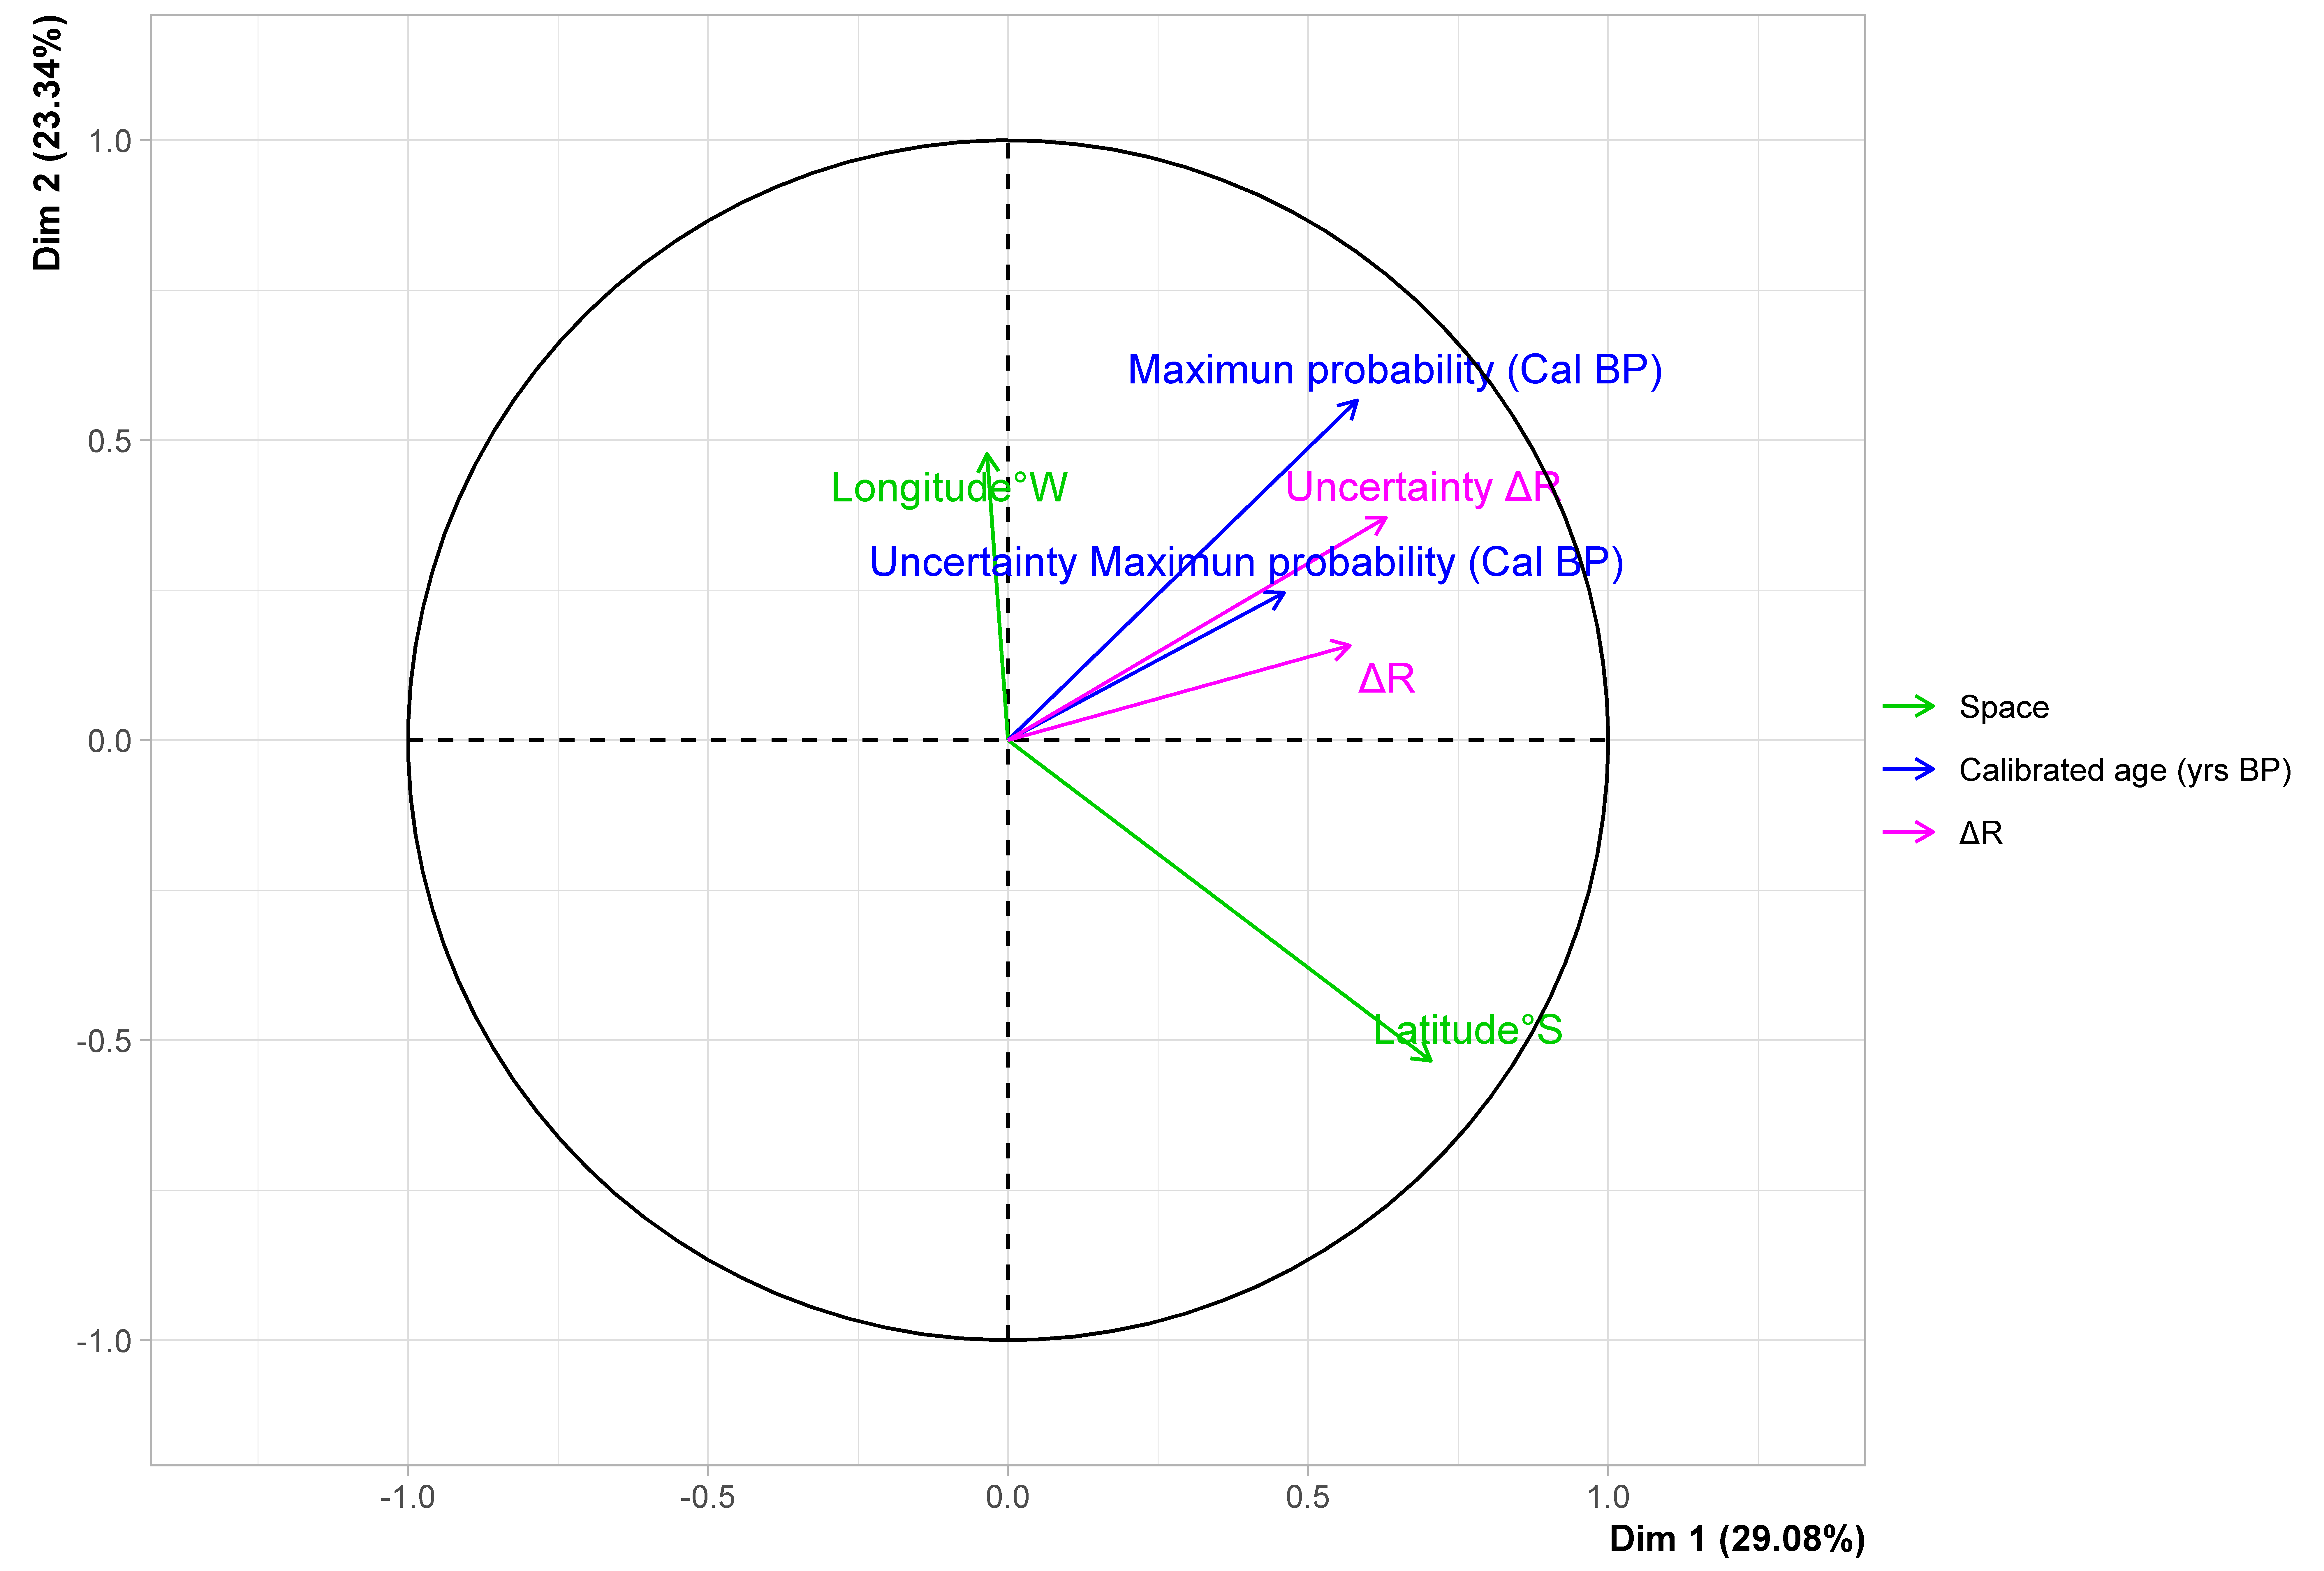
\includegraphics{AMV.biplot.png}}
\end{minipage} \\
\midrule()
\endhead
\emph{Figure 1. Biplot of Principal component of data (n=96)} \\
\bottomrule()
\end{longtable}

PC1 (∼29\%) is interpreted as signal of latitudinal position. PC1 has
the highest loading for latitude, uncertainty of \(\Delta R\) and
calibrated age. PC2 (∼23\%) is interpreted as signal of longitudinal
position. PC2 has the highest loading for calibrated age, longitude and
uncertainty of \(\Delta R\)
\protect\hyperlink{principal-component-analysis-ux28pcaux29}{(fig.~1)}.
Hence, it can be said that the seven variables represent the variability
of the data. My first assumption is to the difference in species or
organic remains is not outstanding for estimating \(\Delta R\).

\hypertarget{clusters-of-local-mra-for-period-time}{%
\subsubsection{Clusters of Local MRA for period
time}\label{clusters-of-local-mra-for-period-time}}

\begin{longtable}[]{@{}
  >{\centering\arraybackslash}p{(\columnwidth - 0\tabcolsep) * \real{1.0000}}@{}}
\toprule()
\begin{minipage}[b]{\linewidth}\centering
\href{https://github.com/jasb3110/Radiocarbon-reservoir/blob/db842ff0620d55ea5ca5ceec0d96a369406b6e3c/plotellipses.period.png?raw=true}{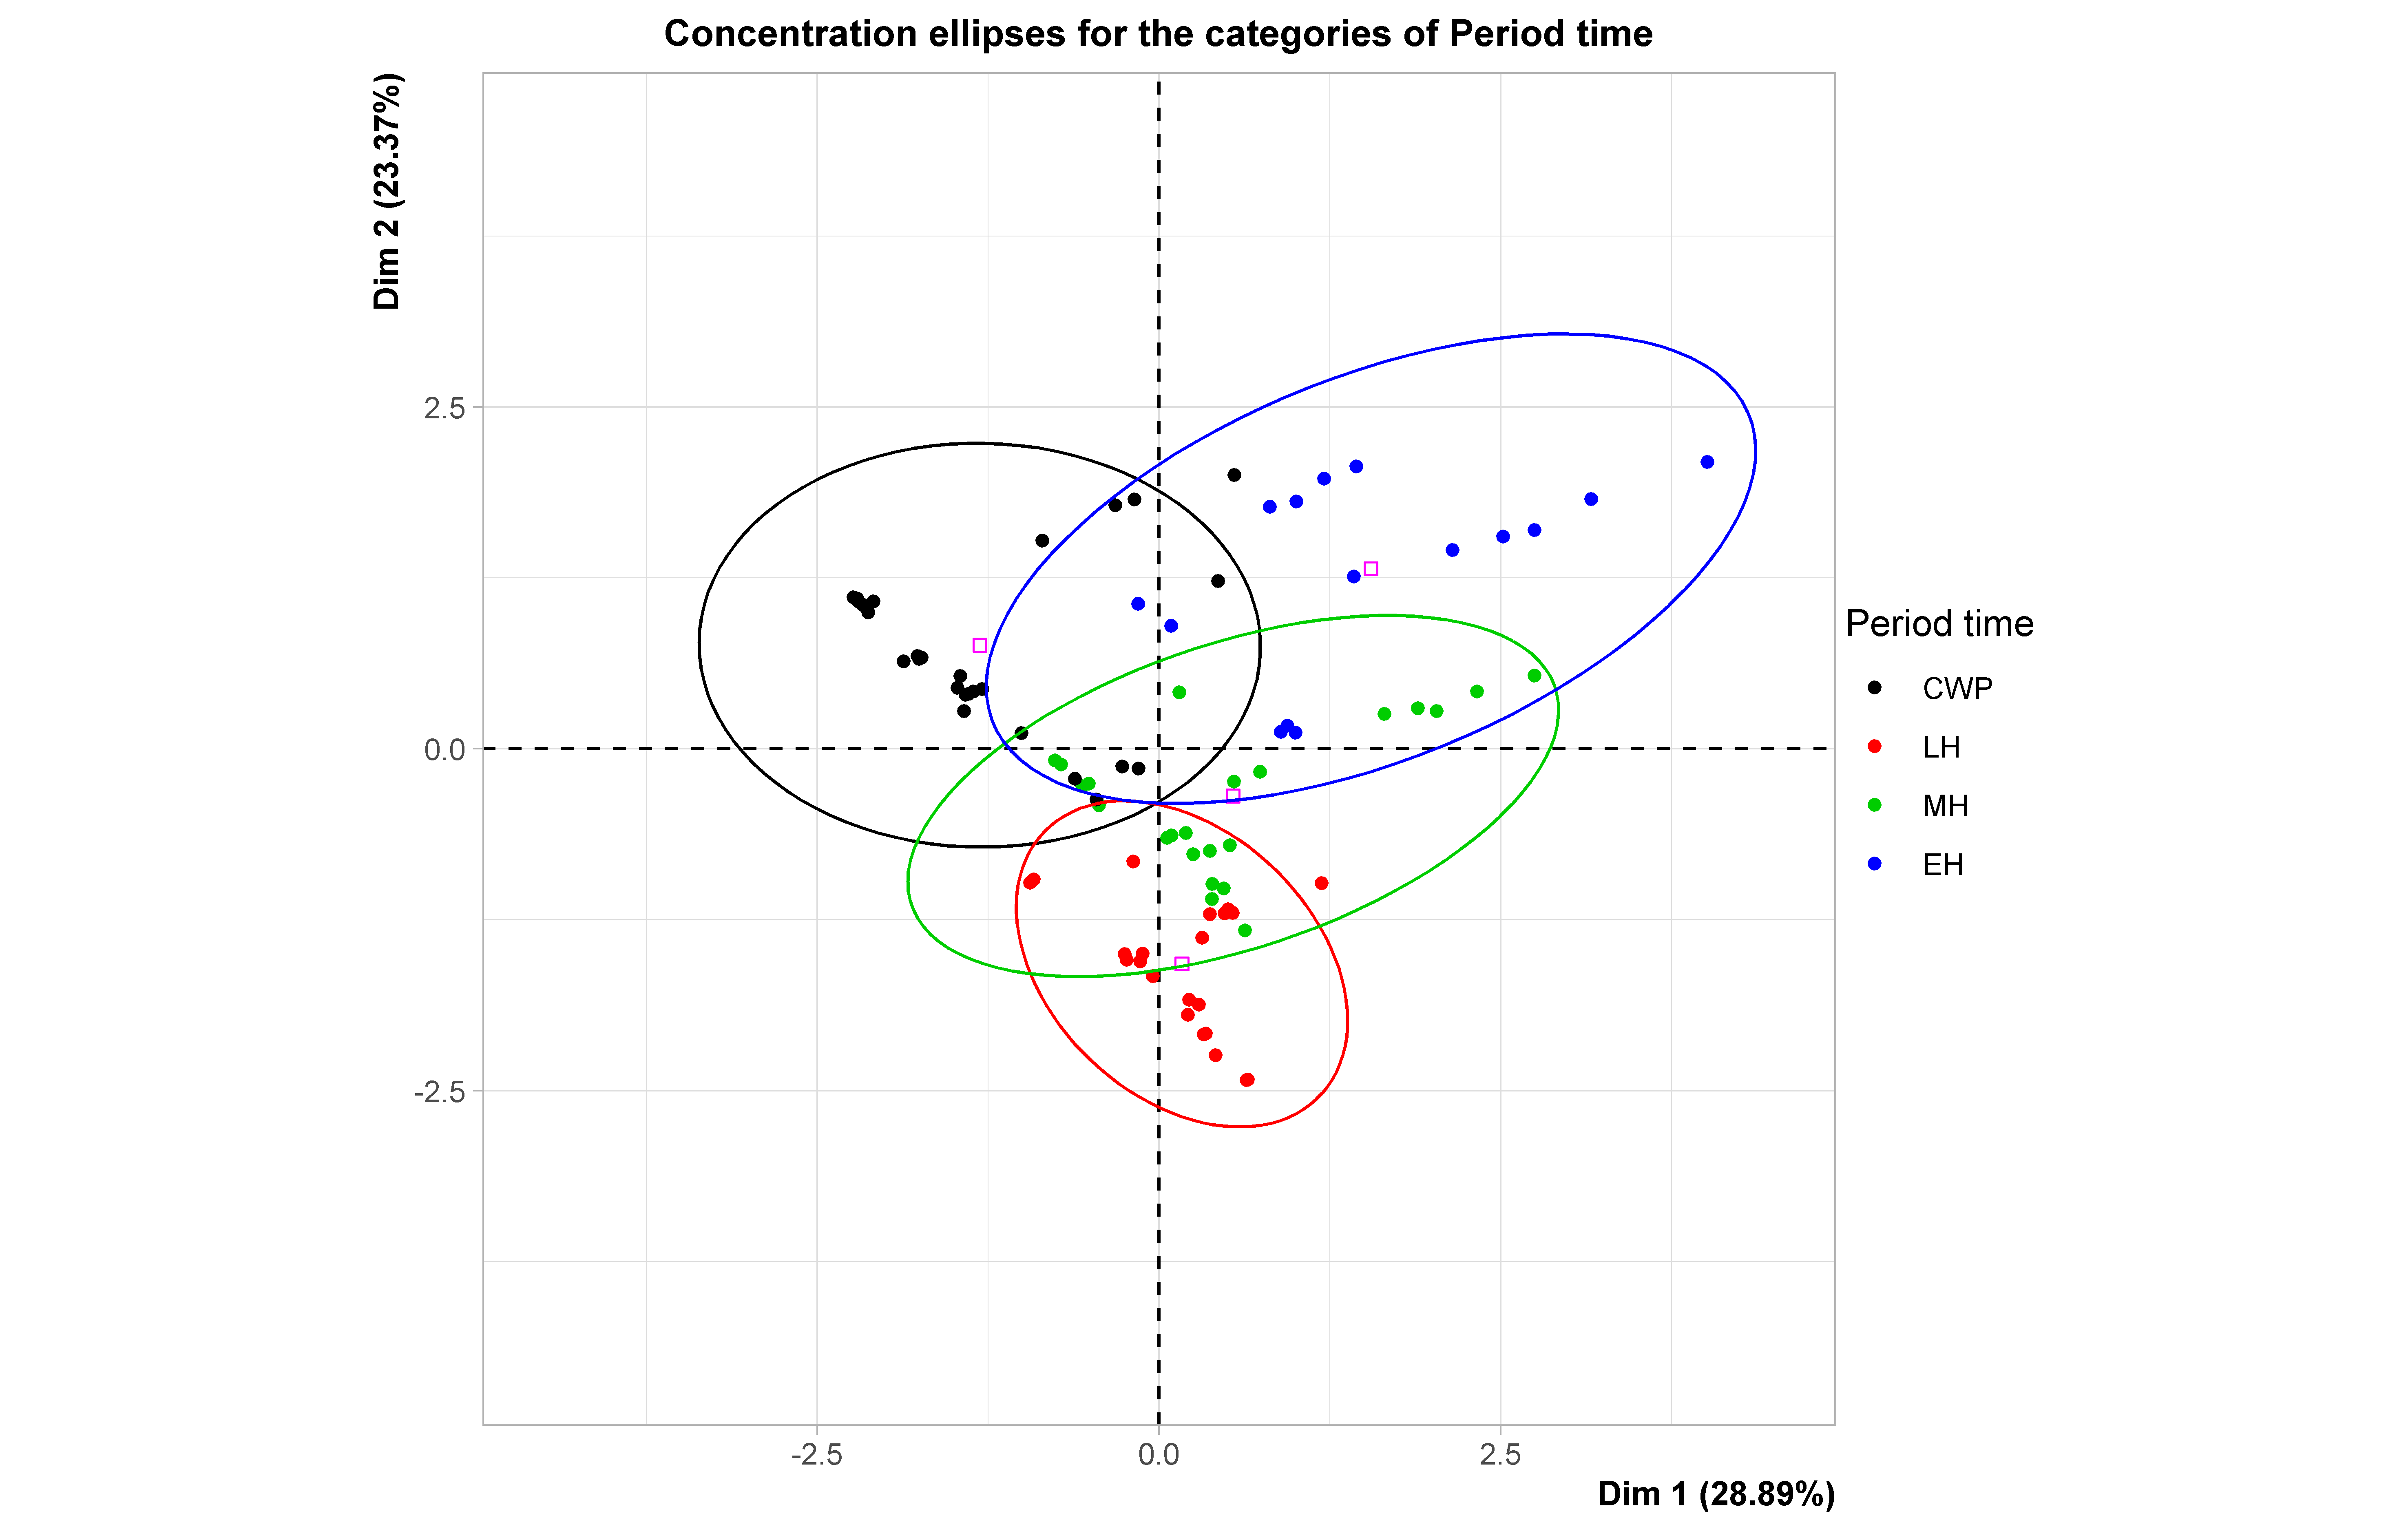
\includegraphics{plotellipses.period.png}}
\end{minipage} \\
\midrule()
\endhead
\emph{Figure 2. Concentration ellipses for the categories of period
time. CWP:Current warming period (black), LH:Late Holocene (red), MH:Mid
Holocene (green), EH:Early Holocene (blue)} \\
\bottomrule()
\end{longtable}

According to periods, It could be no evidence of a temporal effect on
the \(\Delta R\) during the Holocene except for CWP. Therefore, I
noticed a small difference between the periods
\protect\hyperlink{Clusters-of-mra-for-period-time}{(fig.~2)}.
Therefore, we didn't use period-time as an input variable in the model
which will explain forward.

\hypertarget{latitudinal-distribution-of-delta-r-off-peru-to-chile}{%
\subsubsection{\texorpdfstring{Latitudinal distribution of \(\Delta R\)
off Peru to
Chile}{Latitudinal distribution of \textbackslash Delta R off Peru to Chile}}\label{latitudinal-distribution-of-delta-r-off-peru-to-chile}}

Some past works showed the difference in latitudinal of \(\Delta R\) off
Peru to Chile. However, it did not validate a criterion for dividing in
zones before estimating \(\Delta R\).

\begin{figure}
\centering
\includegraphics{https://github.com/jasb3110/Radiocarbon-reservoir/blob/3b3b58adbce85c25b358e8054096a8717a34649d/GAM\%20outcome\%20\%20table.png?raw=true}
\caption{alt text}
\end{figure}

Therefore, I use GAM to find out about the spatial \& temporal effect on
MRA off Peru \& Chile. I built a simple GAM regarding the effects of
individual variables and its interactions (Wood, 2017). This model has
adjusted Tweedie distribution with the logarithm link function and uses
a cubic spline smooth for each variable. According to the output of GAM,
this model has adjusted \(R^{2}\) is 0.83 and desviance explained is
\textasciitilde85\%. hence, this GAM represents the variability of MRA
significantly.

\begin{longtable}[]{@{}
  >{\centering\arraybackslash}p{(\columnwidth - 0\tabcolsep) * \real{1.0000}}@{}}
\toprule()
\begin{minipage}[b]{\linewidth}\centering
\href{https://github.com/jasb3110/Radiocarbon-reservoir/blob/5c906b5d15b85dd72416e0abd3e72d53126c9b7b/GAM\%20radiocarbon\%20heat\%20map.png}{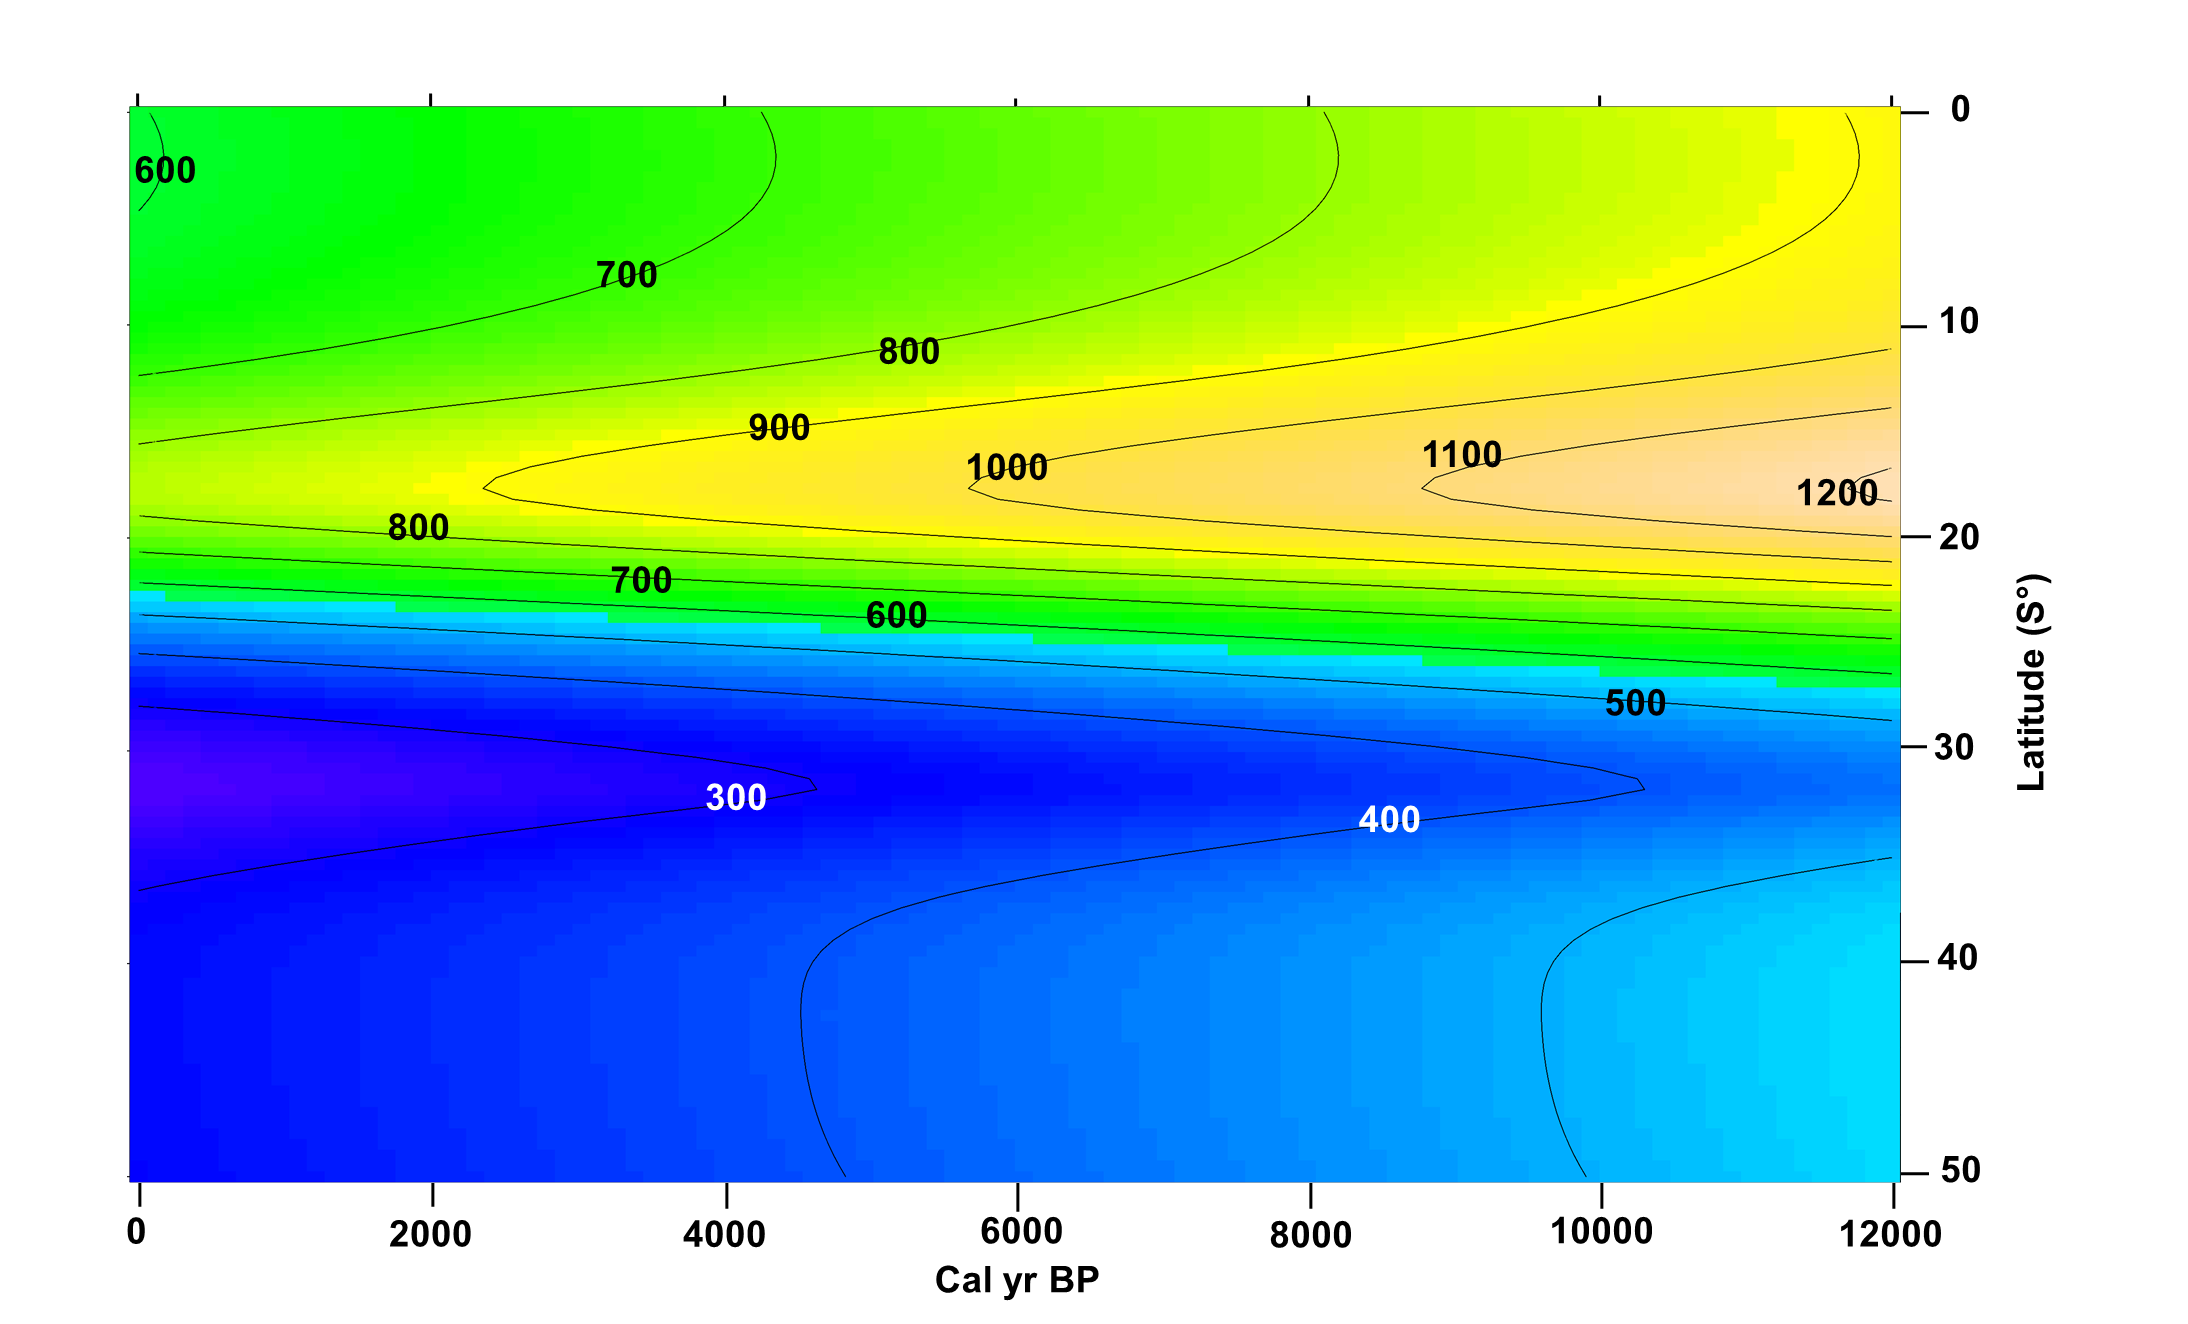
\includegraphics{GAM radiocarbon heat map.png}}
\end{minipage} \\
\midrule()
\endhead
\emph{Figure 3. Latitudinal distribution} \(\Delta R\) \emph{, inferred
for GAM, off Peru to Chile the last 12 Kyr BP} \\
\bottomrule()
\end{longtable}

Then, I plotted \(\Delta R\) GAM, regarding calibrated age and latitude
according to GAM
\protect\hyperlink{latitudinal-distGribution-of-mra-off-peru-to-chile}{(fig.~3)}.
In this picture, I can see a sharp latitudinal pattern which could mean
gradient zone: 17 to 27°S. My second assumption is frontier is 22°S
which mark off two zones: first (0 to 22°S) and second (22 to 50°S). the
limit between the two zones could be due to oceanography and/or
atmosphere change during the last 12 Kyr BP.

\hypertarget{delta-r-estimated-in-boxes-under-marine20}{%
\subsubsection{\texorpdfstring{\(\Delta R\) estimated in boxes under
Marine20}{\textbackslash Delta R estimated in boxes under Marine20}}\label{delta-r-estimated-in-boxes-under-marine20}}

At the state above the latitudinal pattern of \(\Delta R\) split off in
two zones is reliably acceptable. Accordingly, I can estimate
\(\Delta R\) by latitude and periods of time, similar to previous works
\protect\hyperlink{local-mra-estimated-under-marine20}{(fig.~4)}(Carré
etl al, 2016, Ortlieb et al.~2011). The Boxes were built assuming how
\(\Delta R\) is constant within boxes and its frontiers are calculate
one sigma add 5\% more of estimated average \(\Delta R\).

\begin{longtable}[]{@{}
  >{\centering\arraybackslash}p{(\columnwidth - 0\tabcolsep) * \real{1.0000}}@{}}
\toprule()
\begin{minipage}[b]{\linewidth}\centering
\href{https://github.com/jasb3110/Radiocarbon-reservoir/blob/db842ff0620d55ea5ca5ceec0d96a369406b6e3c/MRA.marine20.png?raw=true}{\includegraphics{MRA.marine20.png}}
\end{minipage} \\
\midrule()
\endhead
\emph{Figure 4. Diagram of} \(\Delta R\) \emph{off Peru \& Chile in
boxes. Orange boxes belonged from 0 to 22°S and purple boxes belonged
from 22 to 50°S.The thick black lines is mean value of MRA each box.} \\
\bottomrule()
\end{longtable}

In this picture, I show the estimation of \(\Delta R\) in boxes for two
zones. There are four boxes (two orange and two purple) boxes of
\(\Delta R\) that have belonged to different latitudinal positions and
periods of time (orange boxes: latitude 0-22°S, 10.6 to 5.8 Cal Kyr BP
{[}11.2 to 6.4 Kyr BP{]} and 5.6 to 0.3 Cal Kyr BP {[}6.2 to 0.9 Kyr
BP{]}; purple boxes: latitude 22-50°S, 12 to 6.5 Cal Kyr BP {[}12.6 to
7.05 Kyr BP{]} and 3.4 to 0.1 Cal Kyr BP {[}4 to 0.7 Kyr BP{]}). where
the values with ``{[} {]}'' represents Conventional age interval.

Additionally, We also estimated \(\Delta R\) the last 100 years for
0-22°S and 22-50°S were 140±5 and 162±6, respectively. However, boxes of
CWP was not plotted to avoid overlapping in the picture.

\hypertarget{discussion}{%
\subsection{Discussion}\label{discussion}}

\begin{longtable}[]{@{}
  >{\centering\arraybackslash}p{(\columnwidth - 0\tabcolsep) * \real{1.0000}}@{}}
\toprule()
\begin{minipage}[b]{\linewidth}\centering
\href{https://github.com/jasb3110/Radiocarbon-reservoir/blob/8bddc9b0f2d8f839ca2d4826f47d9050d49384aa/animation.gif?raw=true}{\includegraphics{animation.gif?}}
\end{minipage} \\
\midrule()
\endhead
\emph{Figure 5.Animation of} \(\Delta R\) \emph{off Peru \& Chile in
boxes and MRA in the background, estimated for each calibrated curve how
to difference between Shcal13 \& Marine13 (grey) and Shcal20 \&
Marine20(red). Estimated} \(\Delta R\) \emph{by Ortlieb et
al.~2011(grey); by Carré et al.~2016(green and blue) and by this
work(orange and purple). The thick black lines is the mean value of MRA
each box} \\
\bottomrule()
\end{longtable}

This animation showed comparative principal outcomes of previous works,
and this work\protect\hyperlink{discussion}{(fig.~5)}. The boxes of
\(\Delta R\) are the same pattern as the boxes proposal for Carré et
al.~2016. During EH, the magnitude of \(\Delta R\) was higher in the box
estimated with Marine20 than Marine13 which were estimated for 0-22°s (
\textasciitilde400 years) and 22-50°S (\textasciitilde100 years). In the
same way, during the Mid to Late Holocene, The difference of
\(\Delta R\) can repeat for 0-22°S ( \textasciitilde50 years) and
22-50°S (\textasciitilde100 years).

The difference of \(\Delta R\) could be partially explained for
\(\Delta^{14}C\) deficit average according to Marine13 is
\textasciitilde300 years from 0-10.5 Cal Kyr BP (Reimer et al.~2013) and
according to Marine20 is \textasciitilde500 years from 0-11.6 Cal Kyr BP
(Heaton et al.~2020). But \(\Delta R\) off 0-22° was estimated during EH
which exhibited an excess of \textasciitilde200 years may due to MRA
estimate in Marine20 is coupled to atmospheric \(^{14}C\) and not
Marine13 (Heaton et al.~2020).

During eh, The latitudinal gradient of \(\Delta R\) between boxes 0-22°S
and 22-50°S (\textasciitilde1000 years), also is looking up in this work
\protect\hyperlink{local-mra-estimated-under-marine20}{(fig.~4)}. The
latitudinal gradient of \(\Delta R\) likely was modulated for the minor
contribution of SAMW to EUC and ESSW , has low \(\Delta^{14}C\), in
forming CCW and/or increase upwelling during EH (Carré et al.~2016; Hua
et al.~2016; Ortlieb et al.~2011; Fontugne et al.~2004).

Another hand, The latitudinal gradient of \(\Delta R\) estimated with
GAM model
\protect\hyperlink{latitudinal-distGribution-of-mra-off-peru-to-chile}{(fig.~3)}
showed that the transitional zone between 17 to 27°S probably
interpreted zone of Permanent upwelling moved northward during On
Holocene. Also, it can explain how to increase the input of fresh water
which might contribute to a reduction of the reservoir effect (Merino et
al.~2019).

Additionally, \(\Delta R\) in boxes in this work show that absence of
sample of \textasciitilde6 kyrs BP could be explained which sediments
weren´t recorded in marine sediment for biogeochemistry process for
instance: poor preservation of organic matter, low sedimentation rate
and high coastal erosion due marine transgression.

\hypertarget{conclusions}{%
\subsection{Conclusions}\label{conclusions}}

The spatial variability of \(\Delta R\) could be modulated by three
aspects: 1) Oceanographic changes in associated origin CCW and its
circulation, 2) Enhanced upwelling regionally off SEPO, and 3) Climatic
changes inferred river discharge by precipitation during Holocene in
sourth limit of Humboldt system. Furthermore, a relevant aspect was
decreased uncertainty of \(\Delta R\) for using EWM and bootstrapping
than previous estimations.

Future research should include more variables (e.g marine \(CO_2\) off
Peru to Chile) and calibrated age estimation by others proxies or
methods (e.g Uranium to Thorium rate) to improve the description of the
pattern and will be able to build the best ocean-atmosphere model.

\hypertarget{reference}{%
\subsection{Reference}\label{reference}}

\begin{itemize}
\tightlist
\item
  Alves, E. Q., Macario, K., Ascough, P., \& Bronk Ramsey, C. (2018).
  The Worldwide Marine Radiocarbon Reservoir Effect: Definitions,
  Mechanisms, and Prospects. Reviews of Geophysics, 56(1), 278--305.
  \url{https://doi.org/10.1002/2017RG000588}
\item
  Broecker, W. S., Peng, T. H., Ostlund, G., \& Minze, S. (1985). The
  distribution of bomb Radiocarbon in the ocean. Journal of Geophysical
  Research, 90(C4), 6953 to 6970.
  \url{https://doi.org/http://dx.doi.org/10.1029/JC090iC04p06953}
  -Carré, M., Jackson, D., Maldonado, A., Chase, B. M., \& Sachs, J. P.
  (2016). Variability of 14C reservoir age and air--sea flux of CO2 in
  the Peru--Chile upwelling region during the past 12,000years.
  ELSERVIER Quaternary Research, 7.
  \url{https://doi.org/10.1016/j.yqres.2015.12.002}
\item
  Etayo-Cadavid, M. F., Andrus, C. F. T., Jones, K. B., \& Hodgins, G.
  W. L. (2019). Subseasonal variations in marine reservoir age from
  pre-bomb Donax obesulus and Protothaca asperrima shell carbonate.
  Chemical Geology, 526(June), 110--116.
  \url{https://doi.org/10.1016/j.chemgeo.2018.07.001}
\item
  Fontugne, M., Carré, M., Bentaleb, I., Julien, M., \& Lavallée, D.
  (2004). Radiocarbon reservoir age variations in the south Peruvian
  upwelling during the Holocene. Radiocarbon, 46(2), 531--537.
  \url{https://doi.org/10.1017/S003382220003558X}
\item
  Guiñez, M., Valdés, J., Sifeddine, A., Boussafir, M., \& Dávila, P. M.
  (2014). Anchovy population and ocean-climatic fluctuations in the
  Humboldt Current System during the last 700 years and their
  implications. Palaeogeography, Palaeoclimatology, Palaeoecology, 415,
  210--224. \url{https://doi.org/10.1016/j.palaeo.2014.08.026}
\item
  Gutiérrez, D., Sifeddine, A., Field, D. B., Ortlieb, L., Vargas, G.,
  Chávez, F., Velazco, F., Ferreira, V., Tapia, P., Salvatteci, R.,
  Boucher, H., Morales, M. C., Valdés, J., Reyss, J.-L., Campusano, A.,
  Boussafir, M., Mandeng-Yogo, M., García, M., \& Baumgartner, T.
  (2009). Rapid reorganization in ocean biogeochemistry off Peru towards
  the end of the Little Ice Age. Biogeosciences Discussions, 5(5),
  3919--3943. \url{https://doi.org/10.5194/bgd-5-3919-2008}
\item
  Haslett, J., \& Parnell, A. (2008). A simple monotone process with
  application to radiocarbon-dated depth chronologies. Journal of the
  Royal Statistical Society. Series C: Applied Statistics, 57(4),
  399--418. \url{https://doi.org/10.1111/j.1467-9876.2008.00623.x}
\item
  Heaton, T. J., Köhler, P., Butzin, M., Bard, E., Reimer, R. W.,
  Austin, W. E. N., Bronk Ramsey, C., Grootes, P. M., Hughen, K. A.,
  Kromer, B., Reimer, P. J., Adkins, J., Burke, A., Cook, M. S., Olsen,
  J., \& Skinner, L. C. (2020). Marine20---The Marine Radiocarbon Age
  Calibration Curve (0--55,000 cal BP). Radiocarbon, 62(4), 779--820.
  \url{https://doi.org/10.1017/rdc.2020.68}
\item
  Heaton, T. J., Bard, E., Ramsey, C. B., Hughen, K. A., Köhler, P.,
  Reimer, P. J., Butzin, M., \& Hatté, C. (2022). A RESPONSE TO
  COMMUNITY QUESTIONS ON THE MARINE20 RADIOCARBON AGE CALIBRATION CURVE:
  MARINE RESERVOIR AGES AND THE CALIBRATION OF 14C SAMPLES FROM THE
  OCEANS. Radiocarbon, 00(00), 1--27.
  \url{https://doi.org/https://doi.org/10.1017/RDC.2022.66}
\item
  Hogg, A. G., Heaton, T. J., Hua, Q., Palmer, J. G., Turney, C. S. M.,
  Southon, J., Bayliss, A., Blackwell, P. G., Boswijk, G., Bronk Ramsey,
  C., Pearson, C., Petchey, F., Reimer, P., Reimer, R., \& Wacker, L.
  (2020). SHCal20 Southern Hemisphere Calibration, 0-55,000 Years cal
  BP. Radiocarbon, 62(4), 759--778.
  \url{https://doi.org/10.1017/RDC.2020.59}
\item
  Hua, Q., Webb, G. E., Zhao, J. xin, Nothdurft, L. D., Lybolt, M.,
  Price, G. J., \& Opdyke, B. N. (2015). Large variations in the
  Holocene marine radiocarbon reservoir effect reflect ocean circulation
  and climatic changes. Earth and Planetary Science Letters, 422,
  33--44. \url{https://doi.org/10.1016/j.epsl.2015.03.049}
\item
  Ingram, B. L., \& Southon, J. R. (1996). Reservoir ages in eastern
  Pacific coastal and estuarine waters. Radiocarbon, 38(3), 573--582.
  \url{https://doi.org/10.1017/S0033822200030101}
\item
  Jones, K. B., Hodgins, G. W. L., Dettman, D. L., Andrus, C. F. T.,
  Nelson, A., \& Etayo-Cadavid, M. F. (2007). Seasonal variations in
  Peruvian marine reservoir age from pre-bomb Argopecten purpuratus
  shell carbonate. Radiocarbon, 49(2), 877--888.
  \url{https://doi.org/10.1017/S0033822200042740}
\item
  Kennett, D. J., Ingram, B. L., Southon, J. R., \& Wise, K. (2002).
  Differences in 14C age between stratigraphically associated charcoal
  and marine shell from the Archaic Period site of Kilometer 4, southern
  Peru: Old wood or old water? Radiocarbon, 44(1), 53--58.
  \url{https://doi.org/10.1017/S0033822200064663}
\item
  Merino-Campos, V., De Pol-Holz, R., Southon, J., Latorre, C., \&
  Collado-Fabbri, S. (2019). Marine radiocarbon reservoir age along the
  chilean continental margin. Radiocarbon, 61(1), 195--210.
  \url{https://doi.org/10.1017/RDC.2018.81}
\item
  Ortlieb, L., Vargas, G., \& Saliège, J. F. (2011). Marine radiocarbon
  reservoir effect along the northern Chile-southern Peru coast
  (14-24°S) throughout the Holocene. Quaternary Research, 75(1),
  91--103. \url{https://doi.org/10.1016/j.yqres.2010.07.018}
\item
  Owen, B. D. (2002). Marine carbon reservoir age estimates for the far
  south coast of Peru. Radiocarbon, 44(3), 701--708.
  \url{https://doi.org/10.1017/S003382220003215X}
\item
  Taylor, A. R. E., \& Berger, R. (1967). Radiocarbon Content of Marine
  Shells from the Pacific Coasts of Central and South America. Science,
  158(3805), 1180--1182.
\item
  Toggweiler, J. R., K. Dixon, \& Broecker, W. S. (1991). The Peru
  Upwelling and Ventilatation of the South Pacific Thermocline. New
  York, 96(9), 1--31.
  \url{https://doi.org/https://doi.org/10.1029/91JC02063}
\item
  Reimer, P., Bard, E., Bayliss, A., Beck, J. W., Blackwell, P. G.,
  Ramsey, C. B., Buck, C. E., Cheng, H., Edwards, R. L., Friedrich, M.,
  Grootes, P. M., Guilderson, T. P., Haflidason, H., Hajdas, I., Hatté,
  C., Heaton, T. J., Hoffmann, D. L., Hogg, A. G., Hughen, K. A.,
  \ldots{} Plicht, J. van der. (2013). IntCal13 and Marine13 Radiocarbon
  Age Calibration Curves 0--50,000 Years cal BP. Radiocarbon, 55(4),
  1869--1887. \url{https://doi.org/10.2458/azu_js_rc.55.16947}
\item
  Russell, N., Cook, G. T., Ascough, P. L., Scott, E. M., \& Dugmore, A.
  J. (2011). Examining the inherent variability in ΔR: New methods of
  presenting ΔR values and implications for MRE studies. Radiocarbon,
  53(2), 277--288. \url{https://doi.org/10.1017/s003382220005654x}
\item
  Wood, S.N. (2017). Generalized Additive Models: An Introduction with R
  (2nd ed.). Chapman and Hall/CRC.
  \url{https://doi.org/10.1201/9781315370279}
\end{itemize}

\hypertarget{r-code}{%
\subsection{R code}\label{r-code}}

Bellow I attached a R-script.
\href{mailto:solisbenites.jose@gmail.com}{Contact Us} here, if you
consider to give opinions, suggestions and questions.

\begin{Shaded}
\begin{Highlighting}[]
\NormalTok{\#\#\#\#\#\#\#\#\#\#\#\#\#\#\#\#\#\#\#\#\#\#\#\#\#\#\#\#\#\#\#\#\#\#\#\#\#\#\#\#\#\#\#\#\#\#\#\#\#\#\#\#\#\#\#\#\#\#\#\#\#\#\#\#\#\#\#\#\#\#\#\#\#\#\#\#\#\#\#\#}
\NormalTok{\#to start}

\NormalTok{setwd("\textasciitilde{}/Radiocarbon{-}reservoir/")\#directory}

\NormalTok{library("Bchron")}

\NormalTok{\#To delete outliers}

\NormalTok{d=read.csv("Radiocarbon reservoir.csv",sep=";",dec=".",header = TRUE)\#data all data}
\NormalTok{d=as.data.frame(d)}
\NormalTok{d$label=paste(d$reference,d$Latitude,"°","{-}Material:",d$type.of.material,"Sample:",d$pair,sep=" ")}
\NormalTok{d$curve=d$calibrate.curve}
\NormalTok{d$curve}\CommentTok{[}\OtherTok{d$calibrate.curve=="terrestrial"\&d$Convencial.age\textgreater{}=126}\CommentTok{]}\NormalTok{="shcal20"\#155 ± 11 BP (Hogg et al. 2019) is used in SHCal20.}
\NormalTok{d$curve}\CommentTok{[}\OtherTok{d$calibrate.curve=="marine"}\CommentTok{]}\NormalTok{="Marine20"}
\NormalTok{d$curve}\CommentTok{[}\OtherTok{which(d$calibrate.curve=="terrestrial"\&d$Convencial.age\textless{}126)}\CommentTok{]}\NormalTok{="normal"}
\NormalTok{\#d$curve}\CommentTok{[}\OtherTok{which(d$calibrate.curve=="terrestrial"\&d$Convencial.age\textless{}0)}\CommentTok{]}\NormalTok{="sh3"}
\NormalTok{d$Convencial.age}\CommentTok{[}\OtherTok{which(d$calibrate.curve=="marine"\&d$Convencial.age\textless{}603)}\CommentTok{]}\NormalTok{=604}

\NormalTok{age.t=BchronCalibrate(}
\NormalTok{  ages = d$Convencial.age,}
\NormalTok{  ageSds = d$SD.convencial.age,}
\NormalTok{  eps = 1e{-}05,}
\NormalTok{  calCurves =d$curve,}
\NormalTok{  positions = d$Latitude,}
\NormalTok{  ids=d$label)}

\NormalTok{hafsigma=.382924922548026\#0.382924922548026 }
\NormalTok{onesigma=.682689492137086\#0.682689492137086}
\NormalTok{twosigma=.954499736103642\#0.954499736103642}

\NormalTok{\#p=hafsigma\# half sigma}
\NormalTok{p=onesigma\#one sigma}
\NormalTok{\#p=twosigma\#two sigma}

\NormalTok{d$lower=NULL}
\NormalTok{d$upper=NULL}
\NormalTok{d$max=NULL}
\NormalTok{d$median=NULL}

\NormalTok{vvv=NULL}
\NormalTok{sss=NULL}

\NormalTok{for (i in 1:dim(d)}\CommentTok{[}\OtherTok{1}\CommentTok{]}\NormalTok{)\{}
\NormalTok{  d$mean}\CommentTok{[}\OtherTok{i}\CommentTok{]}\NormalTok{=sum(age.t[}\CommentTok{[}\OtherTok{i}\CommentTok{]}\NormalTok{]$densities*age.t[}\CommentTok{[}\OtherTok{i}\CommentTok{]}\NormalTok{]$ageGrid)}
\NormalTok{  d$median}\CommentTok{[}\OtherTok{i}\CommentTok{]}\NormalTok{=age.t[}\CommentTok{[}\OtherTok{i}\CommentTok{]}\NormalTok{]$ageGrid}\CommentTok{[}\OtherTok{round(length(age.t[[i]}\CommentTok{]}\NormalTok{$densities)*0.5)]}
  
\NormalTok{  if(length(age.t[}\CommentTok{[}\OtherTok{i}\CommentTok{]}\NormalTok{]$ageGrid}\CommentTok{[}\OtherTok{which(age.t[[i]}\CommentTok{]}\NormalTok{$densities==max(age.t[}\CommentTok{[}\OtherTok{i}\CommentTok{]}\NormalTok{]$densities))])==1)\{}
\NormalTok{  d$max}\CommentTok{[}\OtherTok{i}\CommentTok{]}\NormalTok{=age.t[}\CommentTok{[}\OtherTok{i}\CommentTok{]}\NormalTok{]$ageGrid}\CommentTok{[}\OtherTok{which(age.t[[i]}\CommentTok{]}\NormalTok{$densities==max(age.t[}\CommentTok{[}\OtherTok{i}\CommentTok{]}\NormalTok{]$densities))]}
\NormalTok{  \}else\{}
\NormalTok{    vvv=age.t[}\CommentTok{[}\OtherTok{i}\CommentTok{]}\NormalTok{]$ageGrid}\CommentTok{[}\OtherTok{which(age.t[[i]}\CommentTok{]}\NormalTok{$densities==max(age.t[}\CommentTok{[}\OtherTok{i}\CommentTok{]}\NormalTok{]$densities))]}
\NormalTok{    sss= abs(vvv{-}d$mean}\CommentTok{[}\OtherTok{i}\CommentTok{]}\NormalTok{)}
\NormalTok{  d$max}\CommentTok{[}\OtherTok{i}\CommentTok{]}\NormalTok{= vvv}\CommentTok{[}\OtherTok{which(sss==min(sss))}\CommentTok{]}
\NormalTok{  \}}
  
\NormalTok{  if(max(age.t[}\CommentTok{[}\OtherTok{i}\CommentTok{]}\NormalTok{]$ageGrid}\CommentTok{[}\OtherTok{which(cumsum(age.t[[i]}\CommentTok{]}\NormalTok{$densities)\textless{}cumsum(age.t[}\CommentTok{[}\OtherTok{i}\CommentTok{]}\NormalTok{]$densities)}\CommentTok{[}\OtherTok{which(age.t[[i]}\CommentTok{]}\NormalTok{$ageGrid==d$max}\CommentTok{[}\OtherTok{i}\CommentTok{]}\NormalTok{)]{-}p*.5)])=={-}Inf)\{}
\NormalTok{  d$upper}\CommentTok{[}\OtherTok{i}\CommentTok{]}\NormalTok{=min(age.t[}\CommentTok{[}\OtherTok{i}\CommentTok{]}\NormalTok{]$ageGrid)  }
\NormalTok{  \}else\{}
\NormalTok{  d$upper}\CommentTok{[}\OtherTok{i}\CommentTok{]}\NormalTok{=max(age.t[}\CommentTok{[}\OtherTok{i}\CommentTok{]}\NormalTok{]$ageGrid}\CommentTok{[}\OtherTok{which(cumsum(age.t[[i]}\CommentTok{]}\NormalTok{$densities)\textless{}cumsum(age.t[}\CommentTok{[}\OtherTok{i}\CommentTok{]}\NormalTok{]$densities)}\CommentTok{[}\OtherTok{which(age.t[[i]}\CommentTok{]}\NormalTok{$ageGrid==d$max}\CommentTok{[}\OtherTok{i}\CommentTok{]}\NormalTok{)]{-}p*.5)])}
\NormalTok{  \}}
  
\NormalTok{  if(min(age.t[}\CommentTok{[}\OtherTok{i}\CommentTok{]}\NormalTok{]$ageGrid}\CommentTok{[}\OtherTok{which(cumsum(age.t[[i]}\CommentTok{]}\NormalTok{$densities)\textgreater{}cumsum(age.t[}\CommentTok{[}\OtherTok{i}\CommentTok{]}\NormalTok{]$densities)}\CommentTok{[}\OtherTok{which(age.t[[i]}\CommentTok{]}\NormalTok{$ageGrid==d$max}\CommentTok{[}\OtherTok{i}\CommentTok{]}\NormalTok{)]+p*.5)])==Inf)\{}
\NormalTok{  d$lower}\CommentTok{[}\OtherTok{i}\CommentTok{]}\NormalTok{=max(age.t[}\CommentTok{[}\OtherTok{i}\CommentTok{]}\NormalTok{]$ageGrid) }
\NormalTok{  \}else\{}
\NormalTok{  d$lower}\CommentTok{[}\OtherTok{i}\CommentTok{]}\NormalTok{=min(age.t[}\CommentTok{[}\OtherTok{i}\CommentTok{]}\NormalTok{]$ageGrid}\CommentTok{[}\OtherTok{which(cumsum(age.t[[i]}\CommentTok{]}\NormalTok{$densities)\textgreater{}cumsum(age.t[}\CommentTok{[}\OtherTok{i}\CommentTok{]}\NormalTok{]$densities)}\CommentTok{[}\OtherTok{which(age.t[[i]}\CommentTok{]}\NormalTok{$ageGrid==d$max}\CommentTok{[}\OtherTok{i}\CommentTok{]}\NormalTok{)]+p*.5)])}
\NormalTok{  \}}
\NormalTok{  \}}

\NormalTok{d$sdmean.lower=abs(d$lower{-}d$mean)}
\NormalTok{d$sdmean.upper=abs(d$mean{-}d$upper)}

\NormalTok{d$sdmedian.lower=abs(d$lower{-}d$median)}
\NormalTok{d$sdmedian.upper=abs(d$median{-}d$upper)}

\NormalTok{d$sdmax.lower=abs(d$lower{-}d$max)}
\NormalTok{d$sdmax.upper=abs(d$max{-}d$upper)}

\NormalTok{\#for (i in 1:dim(d)}\CommentTok{[}\OtherTok{1}\CommentTok{]}\NormalTok{)\{}
\NormalTok{\#X11();plot(age.t[}\CommentTok{[}\OtherTok{i}\CommentTok{]}\NormalTok{]$ageGrid,age.t[}\CommentTok{[}\OtherTok{i}\CommentTok{]}\NormalTok{]$densities,type="l",xlab="Cal BP",ylab="Density",main =d$label}\CommentTok{[}\OtherTok{i}\CommentTok{]}\NormalTok{)}
\NormalTok{\#abline(v=d$mean}\CommentTok{[}\OtherTok{i}\CommentTok{]}\NormalTok{,col="gray")\#mean value}
\NormalTok{\#abline(v=d$lower}\CommentTok{[}\OtherTok{i}\CommentTok{]}\NormalTok{,col="blue")\# lower value}
\NormalTok{\#abline(v=d$upper}\CommentTok{[}\OtherTok{i}\CommentTok{]}\NormalTok{,col="red")\#upper value}
\NormalTok{\#abline(v=d$median}\CommentTok{[}\OtherTok{i}\CommentTok{]}\NormalTok{,col="green")\#median value}
\NormalTok{\#abline(v=d$max}\CommentTok{[}\OtherTok{i}\CommentTok{]}\NormalTok{,col="black")\#maximum probability value!!!!!!!!!!!!!!!!}
\NormalTok{\#\}}

\NormalTok{\#\#\#\#\#\#\#\#\#\#\#\#\#\#\#\#\#\#\#\#\#\#\#\#\#\#\#\#\#\#\#\#\#\#\#\#\#\#\#\#\#\#\#\#\#\#\#\#\#\#\#\#\#\#\#\#\#\#\#\#\#\#\#\#\#\#\#\#\#\#\#}
\NormalTok{\#Method of Error propagation of variance, according to R.Reimer \& P.Reimer et al. 2016}
\NormalTok{\#according to R.Reimer \& P.Reimer et al. 2016}
\NormalTok{\#Asumption three sample is minimum of pool database}
\NormalTok{\#Error in the weighted mean}

\NormalTok{error.weigthed.mean=function(r,dr,sigma=2,show=1,warning=0,...)\{}
\NormalTok{  if(is.numeric(r)\&\&is.numeric(dr)!=1)\{}
\NormalTok{    stop("Vector values is/are not number(s)") }
\NormalTok{  \}else\{  }
\NormalTok{    if(sum(is.na(r)+is.na(dr))\textgreater{}0)\{}
\NormalTok{      stop("Vector values has NAs") }
\NormalTok{    \}else\{ }
\NormalTok{      if(length(r)/length(dr)!=1)\{ }
\NormalTok{        stop("Vector values are not same size") }
\NormalTok{      \}else\{}
\NormalTok{        if(sum(sigma\textless{}5\&sigma\textgreater{}0)==0)\{}
\NormalTok{          stop("sigma is a value should be major 0 and less 5")}
\NormalTok{        \}else\{}
\NormalTok{          if(length(r)==1)\{}
\NormalTok{            rm=r}
\NormalTok{            delta.r=dr}
\NormalTok{            warn.sign="There is one value, suggesting aggregate more values"}
\NormalTok{          \}else\{    }
\NormalTok{          if(length(r)==2)\{}
\NormalTok{            rm=sum(r/dr\^{}2)/sum( 1/dr\^{}2)}
\NormalTok{            delta.r=sigma*sqrt(1/sum(1/dr\^{}2))}
\NormalTok{            warn.sign="There are two values, suggesting aggregate more values"}
\NormalTok{          \}else\{}
\NormalTok{            rm=sum(r/dr\^{}2)/sum( 1/dr\^{}2)}
\NormalTok{            delta.r =sigma*sqrt((sum(((r{-}rm)/dr)\^{}2)/(length(r){-}1))/(sum((1/dr)\^{}2)/length(r)))}
\NormalTok{            warn.sign=NULL}
\NormalTok{          \}}
\NormalTok{        \}}
\NormalTok{      \}}
\NormalTok{    \}}
\NormalTok{    \}}
\NormalTok{  \}}

\NormalTok{if(sum(warning==TRUE,warning==FALSE,warning==T,warning==F,warning==1,warning==0)==0)\{}
\NormalTok{    stop("if you would see warning: TRUE or T or 1 if you not: FALSE or F or 0") }
\NormalTok{  \}else\{  }
\NormalTok{    if(show==TRUE)\{}
\NormalTok{      print(warn.sign)}
\NormalTok{    \}else\{}
\NormalTok{      invisible()}
\NormalTok{    \}}
\NormalTok{  \}}

\NormalTok{if(sum(show==TRUE,show==FALSE,show==T,show==F,show==1,show==0)==0)\{}
\NormalTok{  stop("if you would see results: TRUE or T or 1 if you not: FALSE or F or 0") }
\NormalTok{  \}else\{  }
\NormalTok{    if(show==TRUE)\{}
\NormalTok{      print(paste0("Mean of Reservoir effect is ",round(rm,0)," and Uncertainty of Reservoir effect is ",round(delta.r,0)))}
\NormalTok{    \}else\{}
\NormalTok{      invisible()}
\NormalTok{    \}}
\NormalTok{  \}}
\NormalTok{outcome=c(rm,delta.r)}
\NormalTok{invisible(outcome)  }
\NormalTok{\}}
\NormalTok{\#\#\#\#\#\#\#\#\#\#\#\#\#\#\#\#\#\#\#\#\#\#\#\#\#\#\#\#\#\#\#\#\#\#\#\#\#\#\#\#\#\#\#\#\#\#\#\#\#\#\#\#\#\#\#\#}
\NormalTok{\#According to Russel et al.2011}
\NormalTok{\#density of R is estimated for bootstrapping ("n")}

\NormalTok{n=1000000\#resamples millon}

\NormalTok{d$calibrate.curve}\CommentTok{[}\OtherTok{d$calibrate.curve=="normal"}\CommentTok{]}\NormalTok{="terrestrial"}

\NormalTok{  funclist=list()}
\NormalTok{  for(i in 1:dim(d)}\CommentTok{[}\OtherTok{1}\CommentTok{]}\NormalTok{)\{}
\NormalTok{    funclist[}\CommentTok{[}\OtherTok{i}\CommentTok{]}\NormalTok{]=assign(paste0("funt",i),approxfun(density(age.t[}\CommentTok{[}\OtherTok{i}\CommentTok{]}\NormalTok{]$densities)))}
\NormalTok{    assign(paste0(d$calibrate.curve}\CommentTok{[}\OtherTok{i}\CommentTok{]}\NormalTok{,i),sample(x=age.t[}\CommentTok{[}\OtherTok{i}\CommentTok{]}\NormalTok{]$ageGrid}\CommentTok{[}\OtherTok{1:length(age.t[[i]}\CommentTok{]}\NormalTok{$densities)],}
\NormalTok{                                                 size =n,}
\NormalTok{                                                 replace=TRUE,}
\NormalTok{                                                 prob = funclist[}\CommentTok{[}\OtherTok{i}\CommentTok{]}\NormalTok{](age.t[}\CommentTok{[}\OtherTok{i}\CommentTok{]}\NormalTok{]$densities}\CommentTok{[}\OtherTok{1:length(age.t[[i]}\CommentTok{]}\NormalTok{$densities)])))}
\NormalTok{  \}}



\NormalTok{\#Estimated reservoir effect each sample}
\NormalTok{\#samples}

\NormalTok{rlist=list()}
\NormalTok{sec=seq(2,dim(d)}\CommentTok{[}\OtherTok{1}\CommentTok{]}\NormalTok{,2)}

\NormalTok{for(i in sec)\{}
\NormalTok{  rlist[}\CommentTok{[}\OtherTok{i}\CommentTok{]}\NormalTok{]=assign(paste0("r",i*.5),get(paste0("marine",i{-}1)){-}get(paste0("terrestrial",i)))}
\NormalTok{\}}

\NormalTok{t.r=as.data.frame(cbind(as.numeric(d$Latitude}\CommentTok{[}\OtherTok{sec}\CommentTok{]}\NormalTok{),as.numeric(d$Longitude}\CommentTok{[}\OtherTok{sec}\CommentTok{]}\NormalTok{),d$max}\CommentTok{[}\OtherTok{sec}\CommentTok{]}\NormalTok{,d$sdmax.lower}\CommentTok{[}\OtherTok{sec}\CommentTok{]}\NormalTok{*.5+d$sdmax.upper[sec]*.5,NA,NA,d$pairs}\CommentTok{[}\OtherTok{sec}\CommentTok{]}\NormalTok{,d$reference}\CommentTok{[}\OtherTok{sec}\CommentTok{]}\NormalTok{,d$obs}\CommentTok{[}\OtherTok{sec}\CommentTok{]}\NormalTok{,d$period.time}\CommentTok{[}\OtherTok{sec}\CommentTok{]}\NormalTok{))}

\NormalTok{colnames(t.r)=c("Latitude","Longitude","Cal BP(Maximun probability)","error(yr)","R","sdR","pair","reference","obs","period")}

\NormalTok{for(i in 1:length(t.r$Latitude))\{}
\NormalTok{t.r$R}\CommentTok{[}\OtherTok{i}\CommentTok{]}\NormalTok{=as.numeric(round(mean(get(paste0("r",i))),2))}
\NormalTok{t.r$sdR}\CommentTok{[}\OtherTok{i}\CommentTok{]}\NormalTok{=as.numeric(round(sd(get(paste0("r",i))),2))}
\NormalTok{\}}

\NormalTok{label=paste0(t.r$Latitude,"/",t.r$}\InformationTok{\textasciigrave{}Cal BP(Maximun probability)\textasciigrave{}}\NormalTok{,"/",t.r$Longitude)}
\NormalTok{label=factor(label,levels=unique(label))}
\NormalTok{t.r$label=label}

\NormalTok{write.csv(t.r,"outcome.csv",sep=";",dec=".",col.names = TRUE)  }
\NormalTok{\#\#\#\#\#\#\#\#\#}
\FunctionTok{\# repeated sample are merged}
\NormalTok{p2=unique(t.r$label)}
\NormalTok{t.r2=t.r}\CommentTok{[}\OtherTok{1:length(p2),}\CommentTok{]}
\NormalTok{t.r2}\CommentTok{[}\OtherTok{1:length(p2),}\CommentTok{]}\NormalTok{=NA}
\NormalTok{t.r2$label=p2}

\NormalTok{for(i in 1:length(p2))\{}
\NormalTok{t.r2$Latitude}\CommentTok{[}\OtherTok{i}\CommentTok{]}\NormalTok{=t.r$Latitude}\CommentTok{[}\OtherTok{which(t.r$label==t.r2$label[i])}\CommentTok{][1]}
\NormalTok{t.r2$Longitude}\CommentTok{[}\OtherTok{i}\CommentTok{]}\NormalTok{= t.r$Longitude}\CommentTok{[}\OtherTok{which(t.r$label==t.r2$label[i])}\CommentTok{][1]} 
\NormalTok{t.r2$reference}\CommentTok{[}\OtherTok{i}\CommentTok{]}\NormalTok{=t.r$reference}\CommentTok{[}\OtherTok{which(t.r$label==t.r2$label[i])}\CommentTok{][1]} 
\NormalTok{t.r2$obs}\CommentTok{[}\OtherTok{i}\CommentTok{]}\NormalTok{=t.r$obs}\CommentTok{[}\OtherTok{which(t.r$label==t.r2$label[i])}\CommentTok{][1]} 
\NormalTok{t.r2$pair}\CommentTok{[}\OtherTok{i}\CommentTok{]}\NormalTok{=t.r$pair}\CommentTok{[}\OtherTok{which(t.r$label==t.r2$label[i])}\CommentTok{][1]} 
\NormalTok{t.r2$period}\CommentTok{[}\OtherTok{i}\CommentTok{]}\NormalTok{=t.r$period}\CommentTok{[}\OtherTok{which(t.r$label==t.r2$label[i])}\CommentTok{][1]} 
\NormalTok{t.r2$}\InformationTok{\textasciigrave{}Cal BP(Maximun probability)\textasciigrave{}}\CommentTok{[}\OtherTok{i}\CommentTok{]}\NormalTok{=t.r$}\InformationTok{\textasciigrave{}Cal BP(Maximun probability)\textasciigrave{}}\CommentTok{[}\OtherTok{which(t.r$label==t.r2$label[i])}\CommentTok{][1]} 
\NormalTok{t.r2$}\InformationTok{\textasciigrave{}error(yr)\textasciigrave{}}\CommentTok{[}\OtherTok{i}\CommentTok{]}\NormalTok{=t.r$}\InformationTok{\textasciigrave{}error(yr)\textasciigrave{}}\CommentTok{[}\OtherTok{which(t.r$label==t.r2$label[i])}\CommentTok{][1]} 
\NormalTok{t.r2$R}\CommentTok{[}\OtherTok{i}\CommentTok{]}\NormalTok{=error.weigthed.mean(as.numeric(t.r$R}\CommentTok{[}\OtherTok{which(t.r$label==t.r2$label[i])}\CommentTok{]}\NormalTok{),dr=as.numeric(t.r$sdR}\CommentTok{[}\OtherTok{which(t.r$label==t.r2$label[i])}\CommentTok{]}\NormalTok{),sigma = 1,show = 0,warning = 0)}\CommentTok{[}\OtherTok{1}\CommentTok{]}
\NormalTok{t.r2$sdR}\CommentTok{[}\OtherTok{i}\CommentTok{]}\NormalTok{=error.weigthed.mean(as.numeric(t.r$R}\CommentTok{[}\OtherTok{which(t.r$label==t.r2$label[i])}\CommentTok{]}\NormalTok{),dr=as.numeric(t.r$sdR}\CommentTok{[}\OtherTok{which(t.r$label==t.r2$label[i])}\CommentTok{]}\NormalTok{),sigma = 1,show = 0,warning = 0)}\CommentTok{[}\OtherTok{2}\CommentTok{]}
\NormalTok{\}}

\NormalTok{t.r2$label=NULL}

\NormalTok{write.csv(t.r2,"outcome2.csv",sep=";",dec=".",col.names = TRUE)\# data without repeated samples  }

\NormalTok{\#\#\#\#\#\#\#\#}
\NormalTok{\#0°S{-}22°S during 6000 to 10500 yr BP}
\NormalTok{w={-}22}
\NormalTok{sigma1=1}
\NormalTok{showme=1}
\NormalTok{warn=1}

\NormalTok{Rp1=as.numeric(t.r2$R}\CommentTok{[}\OtherTok{as.numeric(t.r2$Latitude)\textgreater{}w\&as.numeric(t.r2$\textasciigrave{}Cal BP(Maximun probability)\textasciigrave{})\textgreater{}6000\&t.r2$obs!="not relationship"}\CommentTok{]}\NormalTok{)}
\NormalTok{sRp1=as.numeric(t.r2$sdR}\CommentTok{[}\OtherTok{as.numeric(t.r2$Latitude)\textgreater{}w\&as.numeric(t.r2$\textasciigrave{}Cal BP(Maximun probability)\textasciigrave{})\textgreater{}6000\&t.r2$obs!="not relationship"}\CommentTok{]}\NormalTok{)}
\NormalTok{c1=as.numeric(t.r2$}\InformationTok{\textasciigrave{}Cal BP(Maximun probability)\textasciigrave{}}\CommentTok{[}\OtherTok{as.numeric(t.r2$Latitude)\textgreater{}w\&as.numeric(t.r2$\textasciigrave{}Cal BP(Maximun probability)\textasciigrave{})\textgreater{}6000\&t.r2$obs!="not relationship"}\CommentTok{]}\NormalTok{)}
\NormalTok{p1=error.weigthed.mean(Rp1,sRp1,sigma1,showme,warn)}

\NormalTok{\#during 100 to 5500 yr BP}
\NormalTok{Rp2=as.numeric(t.r2$R}\CommentTok{[}\OtherTok{as.numeric(t.r2$Latitude)\textgreater{}w\&as.numeric(t.r2$\textasciigrave{}Cal BP(Maximun probability)\textasciigrave{})\textgreater{}100\&as.numeric(t.r2$\textasciigrave{}Cal BP(Maximun probability)\textasciigrave{})\textless{}5500\&t.r2$obs!="not relationship"}\CommentTok{]}\NormalTok{)}
\NormalTok{sRp2=as.numeric(t.r2$sdR}\CommentTok{[}\OtherTok{as.numeric(t.r2$Latitude)\textgreater{}w\&as.numeric(t.r2$\textasciigrave{}Cal BP(Maximun probability)\textasciigrave{})\textgreater{}100\&as.numeric(t.r2$\textasciigrave{}Cal BP(Maximun probability)\textasciigrave{})\textless{}5500\&t.r2$obs!="not relationship"}\CommentTok{]}\NormalTok{)}
\NormalTok{c2=as.numeric(t.r2$}\InformationTok{\textasciigrave{}Cal BP(Maximun probability)\textasciigrave{}}\CommentTok{[}\OtherTok{as.numeric(t.r2$Latitude)\textgreater{}w\&as.numeric(t.r2$\textasciigrave{}Cal BP(Maximun probability)\textasciigrave{})\textgreater{}100\&as.numeric(t.r2$\textasciigrave{}Cal BP(Maximun probability)\textasciigrave{})\textless{}5500\&t.r2$obs!="not relationship"}\CommentTok{]}\NormalTok{)}
\NormalTok{p2=error.weigthed.mean(Rp2,sRp2,sigma1,showme,warn)}

\NormalTok{\#during 100 to 4000 yr BP}
\NormalTok{\#Rp3=as.numeric(t.r2$R}\CommentTok{[}\OtherTok{as.numeric(t.r2$Latitude)\textgreater{}w\&as.numeric(t.r2$\textasciigrave{}Cal BP(Maximun probability)\textasciigrave{})\textgreater{}100\&as.numeric(t.r2$\textasciigrave{}Cal BP(Maximun probability)\textasciigrave{})\textless{}4000\&t.r2$obs!="not relationship"}\CommentTok{]}\NormalTok{)}
\NormalTok{\#sRp3=as.numeric(t.r2$sdR}\CommentTok{[}\OtherTok{as.numeric(t.r2$Latitude)\textgreater{}w\&as.numeric(t.r2$\textasciigrave{}Cal BP(Maximun probability)\textasciigrave{})\textgreater{}100\&as.numeric(t.r2$\textasciigrave{}Cal BP(Maximun probability)\textasciigrave{})\textless{}4000\&t.r2$obs!="not relationship"}\CommentTok{]}\NormalTok{)}
\NormalTok{\#error.weigthed.mean(Rp3,sRp3,sigma1,showme,warn)}

\NormalTok{\#during {-}10 to 100 yr BP}
\NormalTok{Rp4=as.numeric(t.r2$R}\CommentTok{[}\OtherTok{as.numeric(t.r2$Latitude)\textgreater{}w\&as.numeric(t.r2$\textasciigrave{}Cal BP(Maximun probability)\textasciigrave{})\textgreater{}{-}10\&as.numeric(t.r2$\textasciigrave{}Cal BP(Maximun probability)\textasciigrave{})\textless{}100\&t.r2$obs!="not relationship"}\CommentTok{]}\NormalTok{)}
\NormalTok{sRp4=as.numeric(t.r2$sdR}\CommentTok{[}\OtherTok{as.numeric(t.r2$Latitude)\textgreater{}w\&as.numeric(t.r2$\textasciigrave{}Cal BP(Maximun probability)\textasciigrave{})\textgreater{}{-}10\&as.numeric(t.r2$\textasciigrave{}Cal BP(Maximun probability)\textasciigrave{})\textless{}100\&t.r2$obs!="not relationship"}\CommentTok{]}\NormalTok{)}
\NormalTok{c3=as.numeric(t.r2$}\InformationTok{\textasciigrave{}Cal BP(Maximun probability)\textasciigrave{}}\CommentTok{[}\OtherTok{as.numeric(t.r2$Latitude)\textgreater{}w\&as.numeric(t.r2$\textasciigrave{}Cal BP(Maximun probability)\textasciigrave{})\textgreater{}{-}10\&as.numeric(t.r2$\textasciigrave{}Cal BP(Maximun probability)\textasciigrave{})\textless{}100\&t.r2$obs!="not relationship"}\CommentTok{]}\NormalTok{)}
\NormalTok{p3=error.weigthed.mean(Rp4,sRp4,sigma1,showme,warn)}

\NormalTok{\#{-}22°S{-}51°S}
\NormalTok{\#during 6000 to 10500 yr BP}
\NormalTok{Rp5=as.numeric(t.r2$R}\CommentTok{[}\OtherTok{as.numeric(t.r2$Latitude)\textless{}w\&as.numeric(t.r2$\textasciigrave{}Cal BP(Maximun probability)\textasciigrave{})\textgreater{}6000}\CommentTok{]}\NormalTok{)}
\NormalTok{sRp5=as.numeric(t.r2$sdR}\CommentTok{[}\OtherTok{as.numeric(t.r2$Latitude)\textless{}w\&as.numeric(t.r2$\textasciigrave{}Cal BP(Maximun probability)\textasciigrave{})\textgreater{}6000}\CommentTok{]}\NormalTok{)}
\NormalTok{c4=as.numeric(t.r2$}\InformationTok{\textasciigrave{}Cal BP(Maximun probability)\textasciigrave{}}\CommentTok{[}\OtherTok{as.numeric(t.r2$Latitude)\textless{}w\&as.numeric(t.r2$\textasciigrave{}Cal BP(Maximun probability)\textasciigrave{})\textgreater{}6000}\CommentTok{]}\NormalTok{)}
\NormalTok{p4=error.weigthed.mean(Rp5,sRp5,sigma1,showme,warn)}

\NormalTok{\#during 100 to 5500 yr BP}
\NormalTok{Rp6=as.numeric(t.r2$R}\CommentTok{[}\OtherTok{as.numeric(t.r2$Latitude)\textless{}w\&as.numeric(t.r2$\textasciigrave{}Cal BP(Maximun probability)\textasciigrave{})\textgreater{}100\&as.numeric(t.r2$\textasciigrave{}Cal BP(Maximun probability)\textasciigrave{})\textless{}5500\&t.r2$obs!="not relationship"}\CommentTok{]}\NormalTok{)}
\NormalTok{sRp6=as.numeric(t.r2$sdR}\CommentTok{[}\OtherTok{as.numeric(t.r2$Latitude)\textless{}w\&as.numeric(t.r2$\textasciigrave{}Cal BP(Maximun probability)\textasciigrave{})\textgreater{}100\&as.numeric(t.r2$\textasciigrave{}Cal BP(Maximun probability)\textasciigrave{})\textless{}5500\&t.r2$obs!="not relationship"}\CommentTok{]}\NormalTok{)}
\NormalTok{c5=as.numeric(t.r2$}\InformationTok{\textasciigrave{}Cal BP(Maximun probability)\textasciigrave{}}\CommentTok{[}\OtherTok{as.numeric(t.r2$Latitude)\textless{}w\&as.numeric(t.r2$\textasciigrave{}Cal BP(Maximun probability)\textasciigrave{})\textgreater{}100\&as.numeric(t.r2$\textasciigrave{}Cal BP(Maximun probability)\textasciigrave{})\textless{}5500\&t.r2$obs!="not relationship"}\CommentTok{]}\NormalTok{)}
\NormalTok{p5=error.weigthed.mean(Rp6,sRp6,sigma1,showme,warn)}

\NormalTok{\#during {-}10 to 100 yr BP}
\NormalTok{Rp8=as.numeric(t.r2$R}\CommentTok{[}\OtherTok{as.numeric(t.r2$Latitude)\textless{}w\&as.numeric(t.r2$\textasciigrave{}Cal BP(Maximun probability)\textasciigrave{})\textgreater{}{-}10\&as.numeric(t.r2$\textasciigrave{}Cal BP(Maximun probability)\textasciigrave{})\textless{}100\&t.r2$obs!="not relationship"}\CommentTok{]}\NormalTok{)}
\NormalTok{sRp8=as.numeric(t.r2$sdR}\CommentTok{[}\OtherTok{as.numeric(t.r2$Latitude)\textless{}w\&as.numeric(t.r2$\textasciigrave{}Cal BP(Maximun probability)\textasciigrave{})\textgreater{}{-}10\&as.numeric(t.r2$\textasciigrave{}Cal BP(Maximun probability)\textasciigrave{})\textless{}100\&t.r2$obs!="not relationship"}\CommentTok{]}\NormalTok{)}
\NormalTok{c6=as.numeric(t.r2$}\InformationTok{\textasciigrave{}Cal BP(Maximun probability)\textasciigrave{}}\CommentTok{[}\OtherTok{as.numeric(t.r2$Latitude)\textless{}w\&as.numeric(t.r2$\textasciigrave{}Cal BP(Maximun probability)\textasciigrave{})\textgreater{}{-}10\&as.numeric(t.r2$\textasciigrave{}Cal BP(Maximun probability)\textasciigrave{})\textless{}100\&t.r2$obs!="not relationship"}\CommentTok{]}\NormalTok{)}
\NormalTok{p6=error.weigthed.mean(Rp8,sRp8,sigma1,showme,warn)}

\NormalTok{\#\#\#\#\#\#\#\#\#\#\#\#\#\#\#\#\#\#\#\#\#\#\#\#\#\#\#\#\#\#\#\#}
\NormalTok{\#Multivariate analysis}
\NormalTok{\#Factominer}
\NormalTok{library("FactoMineR")}
\NormalTok{library("vegan")}
\NormalTok{library("mgcv")}
\NormalTok{library("mgcViz")}
\NormalTok{library("gganimate")}
\NormalTok{library("gamm4")}
\NormalTok{library("mgcViz")}

\NormalTok{t.r2=t.r2}\CommentTok{[}\OtherTok{t.r2$obs!="not relationship",}\CommentTok{]}

\NormalTok{t.r2$period}\CommentTok{[}\OtherTok{t.r2$\textasciigrave{}Cal BP(Maximun probability)\textasciigrave{}\textgreater{}7000}\CommentTok{]}\NormalTok{="EH"}
\NormalTok{t.r2$period}\CommentTok{[}\OtherTok{t.r2$\textasciigrave{}Cal BP(Maximun probability)\textasciigrave{}\textgreater{}4000\&t.r2$\textasciigrave{}Cal BP(Maximun probability)\textasciigrave{}\textless{}7000}\CommentTok{]}\NormalTok{="MH"}
\NormalTok{t.r2$period}\CommentTok{[}\OtherTok{t.r2$\textasciigrave{}Cal BP(Maximun probability)\textasciigrave{}\textgreater{}200\&t.r2$\textasciigrave{}Cal BP(Maximun probability)\textasciigrave{}\textless{}4000}\CommentTok{]}\NormalTok{="LH"}
\NormalTok{t.r2$period}\CommentTok{[}\OtherTok{t.r2$\textasciigrave{}Cal BP(Maximun probability)\textasciigrave{}\textless{}200}\CommentTok{]}\NormalTok{="CWP"}

\NormalTok{sp=t.r2}\CommentTok{[}\OtherTok{,c(1,2)}\CommentTok{]}
\NormalTok{dat=t.r2}\CommentTok{[}\OtherTok{,c(3,4)}\CommentTok{]}
\NormalTok{reser=t.r2}\CommentTok{[}\OtherTok{,c(5,6)}\CommentTok{]}
\NormalTok{\#ref=factor(t.r2$obs,levels=unique(t.r2$obs))}
\NormalTok{ref=factor(t.r2$period,levels=c("CWP","LH","MH","EH"))}

\NormalTok{tab\textless{}{-} data.frame(ref,sp,dat,reser)}

\NormalTok{tab$Latitude=as.numeric(t.r2$Latitude)}
\NormalTok{tab$Longitude=as.numeric(t.r2$Longitude)}
\NormalTok{tab$Cal.BP.Maximun.probability.=as.numeric(tab$Cal.BP.Maximun.probability.)}
\NormalTok{tab$error.yr.=as.numeric(tab$error.yr.)}
\NormalTok{tab$R=as.numeric(tab$R)}
\NormalTok{tab$sdR=as.numeric(tab$sdR)}

\NormalTok{colnames(tab)=c("Period time","Latitude°S",}
\NormalTok{                "Longitude°W","Maximun probability (Cal yr BP)",}
\NormalTok{                "Uncertainty Maximun probability (Cal yr BP)",}
\NormalTok{                expression("\textbackslash{}u0394R"),}
\NormalTok{                paste0("Uncertainty ",expression("\textbackslash{}u0394R")))}
              
\NormalTok{gr\textless{}{-} c(1,ncol(sp),ncol(dat),ncol(reser))}

\NormalTok{t.mfa \textless{}{-} MFA(tab,}
\NormalTok{             group = gr,}
\NormalTok{             type = c("n","c","c","c"),}
\NormalTok{             ncp =,}
\NormalTok{             name.group = c("Period time","Space","Calibrated age (yr BP)","\textbackslash{}u0394R"),}
\NormalTok{             graph =FALSE)}

\FunctionTok{\# Plot the results}
\NormalTok{MFA1=plot(t.mfa,}
\NormalTok{          choix = "axes",}
\NormalTok{          habillage = "group",}
\NormalTok{          shadowtext = TRUE)}

\NormalTok{ggsave("AMV.dimesiones.png", dpi = 900,   width = 250,}
\NormalTok{       height = 159,unit="mm",plot =MFA1)}

\NormalTok{\#x11();plot(}
\NormalTok{\#t.mfa,}
\NormalTok{\#choix = "ind",}
\NormalTok{\#partial = "all",}
\NormalTok{\#habillage = "group")}

\NormalTok{MFA2=plot(t.mfa,}
\NormalTok{          choix = "var",}
\NormalTok{          habillage = "group",}
\NormalTok{          graph.type = "ggplot",}
\NormalTok{          shadowtext =TRUE)}
\NormalTok{\#x11();MFA2}

\NormalTok{ggsave("AMV.biplot.png", dpi = 900,   width = 250,}
\NormalTok{       height = 159,unit="mm",plot =MFA2)}

\NormalTok{MFA3=plot(t.mfa, choix = "group")}
\NormalTok{ggsave("AMV.grupos.png", dpi = 600,   width = 250,}
\NormalTok{       height = 159,unit="mm",plot =MFA3)}

\FunctionTok{\# Eigenvalues, screen plot and broken stick model}
\NormalTok{source (\textquotesingle{}https://raw.githubusercontent.com/zdealveindy/anadat{-}r/master/scripts/NumEcolR2/screestick.R\textquotesingle{})}
\NormalTok{ev\textless{}{-} t.mfa$eig}\CommentTok{[}\OtherTok{, 1}\CommentTok{]}
\NormalTok{names(ev) \textless{}{-} paste("MFA", 1 : length(ev))}

\NormalTok{png("Eigenvalues.stick.png", width = 250, height = 159, units = \textquotesingle{}mm\textquotesingle{}, res =600)}
\NormalTok{screestick(ev, las = 3)}
\NormalTok{dev.off()}

\NormalTok{\#cross{-}relation}
\NormalTok{pvalue \textless{}{-} t.mfa$group$RV}
\NormalTok{pvalue}
\NormalTok{contr=t.mfa$group$contrib}
\NormalTok{contr}
\NormalTok{corrr=t.mfa$group$correlation}
\NormalTok{corrr}

\FunctionTok{\#\# Not run: }
\FunctionTok{\#\#\#\# Confidence ellipses around categories per variable}

\NormalTok{png("plotellipses.period.png", width =250, height = 159, units = \textquotesingle{}mm\textquotesingle{}, res =600)}
\NormalTok{plotellipses(t.mfa,keepvar=1,label="none",level=0.95, means=FALSE,graph.type ="ggplot" ,xlim = c({-}4.5,4.5),ylim = c({-}4.5,4.5))}
\NormalTok{dev.off()}

\NormalTok{\#\#\#\#\#\#\#\#\#\#\#\#\#\#\#\#\#\#\#\#\#\#\#\#\#\#\#\#\#\#\#\#\#\#\#\#\#\#\#\#\#\#\#\#\#\#\#\#\#\#\#\#\#\#\#\#\#\#\#\#\#\#\#\#\#\#\#\#\#\#\#\#\#\#\#\#\#\#\#\#}
\NormalTok{\#data with replicated value}

\NormalTok{rd=t.r}
\NormalTok{colnames(rd)=c("la","lo","cal","e","r","sdr","pair","ref","obs","period","label")}

\NormalTok{rd$r=as.numeric(t.r$R)+1{-}min(as.numeric(t.r$R))}
\NormalTok{rd$sdr=as.numeric(t.r$sdR)}
\NormalTok{rd$la={-}1*as.numeric(t.r$Latitude)}
\NormalTok{rd$lo={-}1*as.numeric(t.r$Longitude)}
\NormalTok{rd$e=as.numeric(t.r$}\InformationTok{\textasciigrave{}error(yr)\textasciigrave{}}\NormalTok{)}
\NormalTok{rd$cal=as.numeric(t.r$}\InformationTok{\textasciigrave{}Cal BP(Maximun probability)\textasciigrave{}}\NormalTok{)+1{-}min(as.numeric(t.r$}\InformationTok{\textasciigrave{}Cal BP(Maximun probability)\textasciigrave{}}\NormalTok{))}
\NormalTok{rd=as.data.frame(rd)}
\NormalTok{rd$label=factor(rd$label,levels=unique(rd$label))}

\NormalTok{\#data without replicated value}

\NormalTok{r.d=t.r2}
\NormalTok{colnames(r.d)=c("la","lo","cal","e","r","sdr","ref")}

\NormalTok{\#library(bestNormalize)}
\NormalTok{\#bestNormalize(as.numeric(t.r2$R))}
\NormalTok{\#r.d$r.norm=predict(orderNorm(as.numeric(t.r2$R)))}
\NormalTok{\#hist(r.d$r.norm)}
\NormalTok{\#hist(as.numeric(t.r2$R))}

\NormalTok{r.d$r=as.numeric(t.r2$R)+1{-}min(as.numeric(t.r2$R))}
\NormalTok{r.d$sdr=as.numeric(t.r2$sdR)}
\NormalTok{r.d$la={-}1*as.numeric(t.r2$Latitude)}
\NormalTok{r.d$lo={-}1*as.numeric(t.r2$Longitude)}
\NormalTok{r.d$e=as.numeric(t.r2$}\InformationTok{\textasciigrave{}error(yr)\textasciigrave{}}\NormalTok{)}
\NormalTok{r.d$cal=as.numeric(t.r2$}\InformationTok{\textasciigrave{}Cal BP(Maximun probability)\textasciigrave{}}\NormalTok{)+1{-}min(as.numeric(t.r2$}\InformationTok{\textasciigrave{}Cal BP(Maximun probability)\textasciigrave{}}\NormalTok{))}
\NormalTok{r.d=as.data.frame(r.d)}
\NormalTok{\#\#\#\#\#\#\#\#\#\#\#\#\#\#\#\#\#\#\#\#\#\#\#\#\#\#\#\#\#\#\#\#\#\#\#\#\#\#\#\#\#\#\#\#\#\#\#\#\#\#\#\#\#\#\#\#\#\#\#\#\#\#\#\#\#\#\#\#\#\#\#\#\#\#\#\#\#\#\#}
\NormalTok{\#GAM for radiocarbon effect on Peru }
\NormalTok{\#Wood et al. 2017}

\NormalTok{r.effect.gam\textless{}{-}gam(r\textasciitilde{}s(la,lo)+s(cal)+s(e)+s(cal,e),family =tw,data =r.d)}

\NormalTok{png("r.gam.check.plot.png", width = 250, height = 159, units = \textquotesingle{}mm\textquotesingle{}, res =600)}
\NormalTok{par(mfrow = c(2,2))}
\NormalTok{gam.check(r.effect.gam)}
\NormalTok{dev.off()}

\NormalTok{anova(r.effect.gam)}
\NormalTok{summary(r.effect.gam)}

\NormalTok{gam.r=as.data.frame(capture.output(summary(r.effect.gam)))}
\NormalTok{write.csv(gam.r,"gam.r.csv",sep=",",dec=".",row.names = FALSE)}

\NormalTok{r.viz.gam=getViz(r.effect.gam)}
\NormalTok{r.trt.gam \textless{}{-} plot(r.viz.gam, allTerms = T) +theme\_test()}

\NormalTok{png("r.gam.plot.png", width = 250, height = 159, units = \textquotesingle{}mm\textquotesingle{}, res =1200)}
\NormalTok{print(r.trt.gam, pages = 1)}
\NormalTok{dev.off()}

\NormalTok{error.effect.gam\textless{}{-}gam(sdr\textasciitilde{}s(la,lo)+s(cal)+s(e)+s(cal,e),family =tw,data =r.d)}
\NormalTok{summary(error.effect.gam)}
\NormalTok{anova(error.effect.gam)}

\NormalTok{gam.err=as.data.frame(capture.output(summary(error.effect.gam)))}
\NormalTok{write.csv(gam.err,"gam.err.csv",sep=",",dec=".",row.names = FALSE)}

\NormalTok{png("error.gam.check.plot.png", width = 250, height = 159, units = \textquotesingle{}mm\textquotesingle{}, res =600)}
\NormalTok{par(mfrow = c(2,2))}
\NormalTok{gam.check(error.effect.gam)}
\NormalTok{dev.off()}

\NormalTok{error.viz.gam=getViz(error.effect.gam)}
\NormalTok{error.trt.gam \textless{}{-} plot(error.viz.gam, allTerms = T) +theme\_test()}

\NormalTok{png("error.gam.plot.png", width = 500, height = 318, units = \textquotesingle{}mm\textquotesingle{}, res =1200)}
\NormalTok{print(error.trt.gam, pages = 1)}
\NormalTok{dev.off()}

\NormalTok{\#\#\#\#\#\#\#\#\#\#\#\#\#}
\NormalTok{library("itsadug")}
\NormalTok{library("visreg")}

\NormalTok{png("R.reservoir.png", width = 500, height = 318, units = \textquotesingle{}mm\textquotesingle{}, res =900)}
\NormalTok{fvisgam(r.effect.gam,n.grid =100,color="topo", view=c("cal","la"),ylim=c(0,50),xlim =c(0,12000),nCol=100,show.diff =FALSE,hide.label = TRUE,rm.ranef=TRUE,transform = "exp", print.summary=FALSE, labcex=0.1,alpha.diff = 0.05,xlab="Calibrated age (Kyrs BP)",ylab="Latitude °S")\#without label}
\NormalTok{dev.off()}

\NormalTok{fvisgam(r.effect.gam,n.grid =100,color="topo", view=c("cal","la"),ylim=c(0,50),xlim =c(0,12000),nCol=100,show.diff =FALSE,transform = "exp")\# WITH number label}

\NormalTok{\#\#\#\#\#\#\#\#\#\#\#\#\#\#\#\#\#\#\#\#\#\#\#\#\#\#\#\#\#\#}
\NormalTok{\#to plot graphics}
\NormalTok{toplot=read.csv("comparacion de las curvas de calibracion.csv",sep=";",dec=".",header = TRUE)}
\NormalTok{library(ggplot2)}
\NormalTok{library(ggh4x)}
\NormalTok{library(reprex)}
\NormalTok{library(tidyverse)}

\NormalTok{\#reliable level}
\NormalTok{\#90\% CL=1.645}
\NormalTok{\#95\% CL=1.96}
\NormalTok{\#99\% CL=2.575}

\NormalTok{cl=1.96\#2 sigma}

\NormalTok{m0=.95\#5\% minor than the smallest value}
\NormalTok{mf=1.05\#5\% major than the biggest value}

\NormalTok{toplot$R.Solis.et.al..2022}\CommentTok{[}\OtherTok{1}\CommentTok{]}\NormalTok{=round(p1}\CommentTok{[}\OtherTok{1}\CommentTok{]}\NormalTok{,0)}
\NormalTok{toplot$X1.sigma.sdR.Solis.et.al..2022}\CommentTok{[}\OtherTok{1}\CommentTok{]}\NormalTok{=round(p1}\CommentTok{[}\OtherTok{2}\CommentTok{]}\NormalTok{*.5,0)}
\NormalTok{toplot$X2.sigmas.sdR.Solis.et.al..2022}\CommentTok{[}\OtherTok{1}\CommentTok{]}\NormalTok{=round(p1}\CommentTok{[}\OtherTok{2}\CommentTok{]}\NormalTok{,0)}
\NormalTok{toplot$max.age.solis}\CommentTok{[}\OtherTok{1}\CommentTok{]}\NormalTok{=round(min(c1)*m0,0)}
\NormalTok{toplot$min.age.solis}\CommentTok{[}\OtherTok{1}\CommentTok{]}\NormalTok{=round(max(c1)*mf,0)}

\NormalTok{toplot$R.Solis.et.al..2022}\CommentTok{[}\OtherTok{2}\CommentTok{]}\NormalTok{=round(p2}\CommentTok{[}\OtherTok{1}\CommentTok{]}\NormalTok{,0)}
\NormalTok{toplot$X1.sigma.sdR.Solis.et.al..2022}\CommentTok{[}\OtherTok{2}\CommentTok{]}\NormalTok{=round(p2}\CommentTok{[}\OtherTok{2}\CommentTok{]}\NormalTok{*.5,0)}
\NormalTok{toplot$X2.sigmas.sdR.Solis.et.al..2022}\CommentTok{[}\OtherTok{2}\CommentTok{]}\NormalTok{=round(p2}\CommentTok{[}\OtherTok{2}\CommentTok{]}\NormalTok{,0)}
\NormalTok{toplot$max.age.solis}\CommentTok{[}\OtherTok{2}\CommentTok{]}\NormalTok{=round(min(c2)*m0,0)}
\NormalTok{toplot$min.age.solis}\CommentTok{[}\OtherTok{2}\CommentTok{]}\NormalTok{=round(max(c2)*mf,0)}

\NormalTok{toplot$R.Solis.et.al..2022}\CommentTok{[}\OtherTok{3}\CommentTok{]}\NormalTok{=round(p3}\CommentTok{[}\OtherTok{1}\CommentTok{]}\NormalTok{,0)}
\NormalTok{toplot$X1.sigma.sdR.Solis.et.al..2022}\CommentTok{[}\OtherTok{3}\CommentTok{]}\NormalTok{=round(p3}\CommentTok{[}\OtherTok{2}\CommentTok{]}\NormalTok{*.5,0)}
\NormalTok{toplot$X2.sigmas.sdR.Solis.et.al..2022}\CommentTok{[}\OtherTok{3}\CommentTok{]}\NormalTok{=round(p3}\CommentTok{[}\OtherTok{2}\CommentTok{]}\NormalTok{,0)}
\NormalTok{toplot$max.age.solis}\CommentTok{[}\OtherTok{3}\CommentTok{]}\NormalTok{=round(min(c3)*m0,0)}
\NormalTok{toplot$min.age.solis}\CommentTok{[}\OtherTok{3}\CommentTok{]}\NormalTok{=round(max(c3)*mf,0)}

\NormalTok{toplot$R.Solis.et.al..2022}\CommentTok{[}\OtherTok{4}\CommentTok{]}\NormalTok{=round(p4}\CommentTok{[}\OtherTok{1}\CommentTok{]}\NormalTok{,0)}
\NormalTok{toplot$X1.sigma.sdR.Solis.et.al..2022}\CommentTok{[}\OtherTok{4}\CommentTok{]}\NormalTok{=round(p4}\CommentTok{[}\OtherTok{2}\CommentTok{]}\NormalTok{*.5,0)}
\NormalTok{toplot$X2.sigmas.sdR.Solis.et.al..2022}\CommentTok{[}\OtherTok{4}\CommentTok{]}\NormalTok{=round(p4}\CommentTok{[}\OtherTok{2}\CommentTok{]}\NormalTok{,0)}
\NormalTok{toplot$max.age.solis}\CommentTok{[}\OtherTok{4}\CommentTok{]}\NormalTok{=round(min(c4)*m0,0)}
\NormalTok{toplot$min.age.solis}\CommentTok{[}\OtherTok{4}\CommentTok{]}\NormalTok{=round(max(c4)*mf,0)}

\NormalTok{toplot$R.Solis.et.al..2022}\CommentTok{[}\OtherTok{5}\CommentTok{]}\NormalTok{=round(p5}\CommentTok{[}\OtherTok{1}\CommentTok{]}\NormalTok{,0)}
\NormalTok{toplot$X1.sigma.sdR.Solis.et.al..2022}\CommentTok{[}\OtherTok{5}\CommentTok{]}\NormalTok{=round(p5}\CommentTok{[}\OtherTok{2}\CommentTok{]}\NormalTok{*.5,0)}
\NormalTok{toplot$X2.sigmas.sdR.Solis.et.al..2022}\CommentTok{[}\OtherTok{5}\CommentTok{]}\NormalTok{=round(p5}\CommentTok{[}\OtherTok{2}\CommentTok{]}\NormalTok{,0)}
\NormalTok{toplot$max.age.solis}\CommentTok{[}\OtherTok{5}\CommentTok{]}\NormalTok{=round(min(c5)*m0,0)}
\NormalTok{toplot$min.age.solis}\CommentTok{[}\OtherTok{5}\CommentTok{]}\NormalTok{=round(max(c5)*mf,0)}

\NormalTok{toplot$R.Solis.et.al..2022}\CommentTok{[}\OtherTok{6}\CommentTok{]}\NormalTok{=round(p6}\CommentTok{[}\OtherTok{1}\CommentTok{]}\NormalTok{,0)}
\NormalTok{toplot$X1.sigma.sdR.Solis.et.al..2022}\CommentTok{[}\OtherTok{6}\CommentTok{]}\NormalTok{=round(p6}\CommentTok{[}\OtherTok{2}\CommentTok{]}\NormalTok{*.5,0)}
\NormalTok{toplot$X2.sigmas.sdR.Solis.et.al..2022}\CommentTok{[}\OtherTok{6}\CommentTok{]}\NormalTok{=round(p6}\CommentTok{[}\OtherTok{2}\CommentTok{]}\NormalTok{,0)}
\NormalTok{toplot$max.age.solis}\CommentTok{[}\OtherTok{6}\CommentTok{]}\NormalTok{=round(min(c6)*m0,0)}
\NormalTok{toplot$min.age.solis}\CommentTok{[}\OtherTok{6}\CommentTok{]}\NormalTok{=round(max(c6)*mf,0)}

\NormalTok{\#SHCAL13}
\NormalTok{toplot$min.shcal13=toplot$shcal13{-}toplot$shcal13.sd*cl}
\NormalTok{toplot$max.shcal13=toplot$shcal13+toplot$shcal13.sd*cl}

\NormalTok{\#SHCAL20}
\NormalTok{toplot$min.shcal20=toplot$shcal20{-}toplot$shcal20.sd*cl}
\NormalTok{toplot$max.shcal20=toplot$shcal20+toplot$shcal20.sd*cl}

\NormalTok{\#marine04}
\NormalTok{toplot$min.marine04=toplot$marine04{-}toplot$marine04.sd*cl}
\NormalTok{toplot$max.marine04=toplot$marine04+toplot$marine04.sd*cl}

\NormalTok{\#marine13}
\NormalTok{toplot$min.marine13=toplot$marine13{-}toplot$marine13.sd*cl}
\NormalTok{toplot$max.marine13=toplot$marine13+toplot$marine13.sd*cl}

\NormalTok{\#marine20}
\NormalTok{toplot$min.marine20=toplot$marine20{-}toplot$marine20.sd*cl}
\NormalTok{toplot$max.marine20=toplot$marine20+toplot$marine20.sd*cl}

\NormalTok{error.subs.prop=function(nn=1000000,m1,sd1,m2,sd2)\{}
\NormalTok{out=rnorm(nn,m1,sd1){-}rnorm(nn,m2,sd2)}
\NormalTok{outcome=c(mean(out),sd(out))}
\NormalTok{invisible(outcome)  }
\NormalTok{\}}

\NormalTok{for(i in 1:length(na.omit(toplot$marine13)))\{}
\NormalTok{outy=error.subs.prop(nn = 100000,}
\NormalTok{                    toplot$marine13}\CommentTok{[}\OtherTok{i}\CommentTok{]}\NormalTok{,}
\NormalTok{                    toplot$marine13.sd}\CommentTok{[}\OtherTok{i}\CommentTok{]}\NormalTok{,}
\NormalTok{                    toplot$shcal13}\CommentTok{[}\OtherTok{which(toplot$age.shcal13==toplot$age.marine13[i])}\CommentTok{]}\NormalTok{,}
\NormalTok{                    toplot$shcal13.sd}\CommentTok{[}\OtherTok{which(toplot$age.shcal13==toplot$age.marine13[i])}\CommentTok{]}\NormalTok{)  }
\NormalTok{toplot$MRA.marine13.mean}\CommentTok{[}\OtherTok{i}\CommentTok{]}\NormalTok{=round(outy}\CommentTok{[}\OtherTok{1}\CommentTok{]}\NormalTok{,digits = 0)}
\NormalTok{toplot$MRA.marine13.sd}\CommentTok{[}\OtherTok{i}\CommentTok{]}\NormalTok{  =round(outy}\CommentTok{[}\OtherTok{2}\CommentTok{]}\NormalTok{,digits = 0)}
\NormalTok{\}}

\NormalTok{for(i in 1:length(na.omit(toplot$marine20)))\{}
\NormalTok{  outy=error.subs.prop(nn = 100000,}
\NormalTok{                       toplot$marine20}\CommentTok{[}\OtherTok{i}\CommentTok{]}\NormalTok{,}
\NormalTok{                       toplot$marine20.sd}\CommentTok{[}\OtherTok{i}\CommentTok{]}\NormalTok{,}
\NormalTok{                       toplot$shcal20}\CommentTok{[}\OtherTok{which(toplot$age.shcal20==toplot$age.marine20[i])}\CommentTok{]}\NormalTok{,}
\NormalTok{                       toplot$shcal20.sd}\CommentTok{[}\OtherTok{which(toplot$age.shcal20==toplot$age.marine20[i])}\CommentTok{]}\NormalTok{)  }
\NormalTok{  toplot$MRA.marine20.mean}\CommentTok{[}\OtherTok{i}\CommentTok{]}\NormalTok{=round(outy}\CommentTok{[}\OtherTok{1}\CommentTok{]}\NormalTok{,digits = 0)}
\NormalTok{  toplot$MRA.marine20.sd}\CommentTok{[}\OtherTok{i}\CommentTok{]}\NormalTok{  =round(outy}\CommentTok{[}\OtherTok{2}\CommentTok{]}\NormalTok{,digits = 0)}
\NormalTok{\}}

\NormalTok{toplot$MRA.marine20.max=toplot$MRA.marine20.mean+toplot$MRA.marine20.sd*cl}
\NormalTok{toplot$MRA.marine20.min=toplot$MRA.marine20.mean{-}toplot$MRA.marine20.sd*cl}
\NormalTok{toplot$MRA.marine13.max=toplot$MRA.marine13.mean+toplot$MRA.marine13.sd*cl}
\NormalTok{toplot$MRA.marine13.min=toplot$MRA.marine13.mean{-}toplot$MRA.marine13.sd*cl}

\NormalTok{labely=expression(paste("Radiocarbon age ("\^{}\{14\},"C yr BP)"))}

\NormalTok{labely2=expression(paste("MRA ("\^{}\{14\},"C yr)"))}

\NormalTok{  al=.02}
\NormalTok{  aq=.01}
\NormalTok{  aw=.005}
\NormalTok{  a1="gray"}
\NormalTok{  a2="blue"}
\NormalTok{  a3="green"}
\NormalTok{  a4="red"}
\NormalTok{  a5="orange"}
\NormalTok{  a6="purple"}
\NormalTok{\#\#\#\#\#\#\#\#\#\#\#\#\#\#\#\#\#\#\#\#\#\#}
\NormalTok{\#Zones of another works}
\NormalTok{  toplot$Zone.carre}\CommentTok{[}\OtherTok{1:2}\CommentTok{]}\NormalTok{=as.character("Zone 1: 0{-}24°S")}
\NormalTok{  toplot$Zone.carre}\CommentTok{[}\OtherTok{3:4}\CommentTok{]}\NormalTok{=as.character("Zone 2: 24{-}32°S")}
\NormalTok{  toplot$Zone.ortlieb}\CommentTok{[}\OtherTok{1:4}\CommentTok{]}\NormalTok{=as.character("Zone : 14{-}24°S")}
  
\NormalTok{\#MRA according to Marine20}
\NormalTok{toplot$Zone.solis}\CommentTok{[}\OtherTok{1:3}\CommentTok{]}\NormalTok{=as.character("Zone 1: 0{-}22°S")}
\NormalTok{toplot$Zone.solis}\CommentTok{[}\OtherTok{4:6}\CommentTok{]}\NormalTok{=as.character("Zone 2: 22{-}50°S")}
\NormalTok{t.r2$zone=NA}

\NormalTok{t.r2$Latitude=as.numeric(t.r2$Latitude)}
\NormalTok{t.r2$zone=rep(NA,length(t.r2$Latitude))}
\NormalTok{t.r2$zone}\CommentTok{[}\OtherTok{which(t.r2$Latitude\textgreater{}22*{-}1)}\CommentTok{]}\NormalTok{=as.character("Zone 1: 0{-}22°S")}
\NormalTok{t.r2$zone}\CommentTok{[}\OtherTok{which(t.r2$Latitude\textless{}22*{-}1)}\CommentTok{]}\NormalTok{=as.character("Zone 2: 22{-}50°S")}
\NormalTok{t.r2$zone=factor(t.r2$zone,levels=c("Zone 1: 0{-}22°S","Zone 2: 22{-}50°S"))}

\NormalTok{t.r2$}\InformationTok{\textasciigrave{}Cal BP(Maximun probability)\textasciigrave{}}\NormalTok{=as.numeric(t.r2$}\InformationTok{\textasciigrave{}Cal BP(Maximun probability)\textasciigrave{}}\NormalTok{)}
\NormalTok{t.r2$R=as.numeric(t.r2$R)}
\NormalTok{t.r2$}\InformationTok{\textasciigrave{}error(yr)\textasciigrave{}}\NormalTok{=as.numeric(t.r2$}\InformationTok{\textasciigrave{}error(yr)\textasciigrave{}}\NormalTok{)}
\NormalTok{t.r2$R=as.numeric(t.r2$R)}
\NormalTok{t.r2$sdR=as.numeric(t.r2$sdR)}

\NormalTok{MRA.marine20=ggplot(data =t.r2,aes(x=}\InformationTok{\textasciigrave{}Cal BP(Maximun probability)\textasciigrave{}}\NormalTok{,y=R),size=1)+}

\NormalTok{  geom\_rect(aes(xmin = toplot$min.age.solis}\CommentTok{[}\OtherTok{1}\CommentTok{]}\NormalTok{, }
\NormalTok{                xmax = toplot$max.age.solis}\CommentTok{[}\OtherTok{1}\CommentTok{]}\NormalTok{, }
\NormalTok{                ymin = toplot$R.Solis.et.al..2022}\CommentTok{[}\OtherTok{1}\CommentTok{]}\NormalTok{{-}toplot$X1.sigma.sdR.Solis.et.al..2022}\CommentTok{[}\OtherTok{1}\CommentTok{]}\NormalTok{,}
\NormalTok{                ymax = toplot$R.Solis.et.al..2022}\CommentTok{[}\OtherTok{1}\CommentTok{]}\NormalTok{+toplot$X1.sigma.sdR.Solis.et.al..2022}\CommentTok{[}\OtherTok{1}\CommentTok{]}\NormalTok{),}
\NormalTok{            alpha = aq,}
\NormalTok{            fill = a5)+}
  
\NormalTok{  geom\_rect(aes(xmin = toplot$min.age.solis}\CommentTok{[}\OtherTok{2}\CommentTok{]}\NormalTok{, }
\NormalTok{                xmax = toplot$max.age.solis}\CommentTok{[}\OtherTok{2}\CommentTok{]}\NormalTok{, }
\NormalTok{                ymin = toplot$R.Solis.et.al..2022}\CommentTok{[}\OtherTok{2}\CommentTok{]}\NormalTok{{-}toplot$X1.sigma.sdR.Solis.et.al..2022}\CommentTok{[}\OtherTok{2}\CommentTok{]}\NormalTok{,}
\NormalTok{                ymax = toplot$R.Solis.et.al..2022}\CommentTok{[}\OtherTok{2}\CommentTok{]}\NormalTok{+toplot$X1.sigma.sdR.Solis.et.al..2022}\CommentTok{[}\OtherTok{2}\CommentTok{]}\NormalTok{),}
\NormalTok{            alpha = aq,}
\NormalTok{            fill = a5)+}
 
\NormalTok{  geom\_rect(aes(xmin = toplot$min.age.solis}\CommentTok{[}\OtherTok{4}\CommentTok{]}\NormalTok{, }
\NormalTok{              xmax = toplot$max.age.solis}\CommentTok{[}\OtherTok{4}\CommentTok{]}\NormalTok{, }
\NormalTok{              ymin = toplot$R.Solis.et.al..2022}\CommentTok{[}\OtherTok{4}\CommentTok{]}\NormalTok{{-}toplot$X1.sigma.sdR.Solis.et.al..2022}\CommentTok{[}\OtherTok{4}\CommentTok{]}\NormalTok{,}
\NormalTok{              ymax = toplot$R.Solis.et.al..2022}\CommentTok{[}\OtherTok{4}\CommentTok{]}\NormalTok{+toplot$X1.sigma.sdR.Solis.et.al..2022}\CommentTok{[}\OtherTok{4}\CommentTok{]}\NormalTok{),}
\NormalTok{          alpha = aq,}
\NormalTok{          fill = a6)+}

\NormalTok{  geom\_rect(aes(xmin = toplot$min.age.solis}\CommentTok{[}\OtherTok{5}\CommentTok{]}\NormalTok{, }
\NormalTok{                xmax = toplot$max.age.solis}\CommentTok{[}\OtherTok{5}\CommentTok{]}\NormalTok{, }
\NormalTok{                ymin = toplot$R.Solis.et.al..2022}\CommentTok{[}\OtherTok{5}\CommentTok{]}\NormalTok{{-}toplot$X1.sigma.sdR.Solis.et.al..2022}\CommentTok{[}\OtherTok{5}\CommentTok{]}\NormalTok{,}
\NormalTok{                ymax = toplot$R.Solis.et.al..2022}\CommentTok{[}\OtherTok{5}\CommentTok{]}\NormalTok{+toplot$X1.sigma.sdR.Solis.et.al..2022}\CommentTok{[}\OtherTok{5}\CommentTok{]}\NormalTok{),}
\NormalTok{            alpha = aq,}
\NormalTok{            fill = a6)+}
\NormalTok{  geom\_errorbar(aes(ymin=t.r2$R{-}t.r2$sdR,ymax=t.r2$R+t.r2$sdR),width=5,}
\NormalTok{                            position = position\_dodge(0.5),lwd=.1)+}
\NormalTok{  geom\_errorbarh(aes(xmin=t.r2$}\InformationTok{\textasciigrave{}Cal BP(Maximun probability)\textasciigrave{}}\NormalTok{{-}t.r2$}\InformationTok{\textasciigrave{}error(yr)\textasciigrave{}}\NormalTok{,xmax=t.r2$}\InformationTok{\textasciigrave{}Cal BP(Maximun probability)\textasciigrave{}}\NormalTok{+t.r2$}\InformationTok{\textasciigrave{}error(yr)\textasciigrave{}}\NormalTok{),height=5,}
\NormalTok{              position = position\_dodge(0.5),lwd=.1)+}
\NormalTok{              geom\_point(aes(color=zone),size=2,show.legend =FALSE)+}
  
\NormalTok{  geom\_segment(aes(y =(toplot$R.Solis.et.al..2022}\CommentTok{[}\OtherTok{1}\CommentTok{]}\NormalTok{),}
\NormalTok{                   yend =(toplot$R.Solis.et.al..2022}\CommentTok{[}\OtherTok{1}\CommentTok{]}\NormalTok{),}
\NormalTok{                   x=(toplot$min.age.solis}\CommentTok{[}\OtherTok{1}\CommentTok{]}\NormalTok{),}
\NormalTok{                   xend=toplot$max.age.solis}\CommentTok{[}\OtherTok{1}\CommentTok{]}\NormalTok{),colour="black", size = .75)+}
  
\NormalTok{  geom\_segment(aes(y =(toplot$R.Solis.et.al..2022}\CommentTok{[}\OtherTok{2}\CommentTok{]}\NormalTok{),}
\NormalTok{                   yend =(toplot$R.Solis.et.al..2022}\CommentTok{[}\OtherTok{2}\CommentTok{]}\NormalTok{),}
\NormalTok{                   x=(toplot$min.age.solis}\CommentTok{[}\OtherTok{2}\CommentTok{]}\NormalTok{),}
\NormalTok{                   xend=toplot$max.age.solis}\CommentTok{[}\OtherTok{2}\CommentTok{]}\NormalTok{),colour="black",size = .75)+}
  
\NormalTok{  geom\_segment(aes(y =toplot$R.Solis.et.al..2022}\CommentTok{[}\OtherTok{4}\CommentTok{]}\NormalTok{,}
\NormalTok{                   yend =toplot$R.Solis.et.al..2022}\CommentTok{[}\OtherTok{4}\CommentTok{]}\NormalTok{,}
\NormalTok{                   x=toplot$min.age.solis}\CommentTok{[}\OtherTok{4}\CommentTok{]}\NormalTok{,}
\NormalTok{                   xend=toplot$max.age.solis}\CommentTok{[}\OtherTok{4}\CommentTok{]}\NormalTok{),colour="black", size = .75)+}
  
\NormalTok{  geom\_segment(aes(y =toplot$R.Solis.et.al..2022}\CommentTok{[}\OtherTok{5}\CommentTok{]}\NormalTok{,}
\NormalTok{                   yend =toplot$R.Solis.et.al..2022}\CommentTok{[}\OtherTok{5}\CommentTok{]}\NormalTok{,}
\NormalTok{                   x=toplot$min.age.solis}\CommentTok{[}\OtherTok{5}\CommentTok{]}\NormalTok{,}
\NormalTok{                   xend=toplot$max.age.solis}\CommentTok{[}\OtherTok{5}\CommentTok{]}\NormalTok{),colour="black", size = .75)+}
\NormalTok{  geom\_point(size =1.6, fill ="black", colour = "black",show.legend =FALSE)+}
\NormalTok{  geom\_point(aes(fill= zone,colour=zone),size =1.5,show.legend =FALSE)+}
 
\NormalTok{  annotate("text",x=2000,y=1500,label="\textbackslash{}u0394R Box  0 to 22°S", size = 8,col=a5)+}
\NormalTok{  annotate("text",x=2000,y=1300,label="\textbackslash{}u0394R Box 22 to 50°S", size = 8,col=a6)+}
  
\NormalTok{  annotate("text",x=toplot$min.age.solis}\CommentTok{[}\OtherTok{1}\CommentTok{]}\NormalTok{*.5+toplot$max.age.solis[1]*.5,y=round(toplot$R.Solis.et.al..2022[1]*1.6),label=paste0("\textbackslash{}u0394R=",toplot$R.Solis.et.al..2022}\CommentTok{[}\OtherTok{1}\CommentTok{]}\NormalTok{,"\textbackslash{}u00b1",toplot$X1.sigma.sdR.Solis.et.al..2022}\CommentTok{[}\OtherTok{1}\CommentTok{]}\NormalTok{), size = 6)+}
\NormalTok{  annotate("text",x=toplot$min.age.solis}\CommentTok{[}\OtherTok{2}\CommentTok{]}\NormalTok{*.5+toplot$max.age.solis[2]*.5,y=round(toplot$R.Solis.et.al..2022[2]*2.1),label=paste0("\textbackslash{}u0394R=",toplot$R.Solis.et.al..2022}\CommentTok{[}\OtherTok{2}\CommentTok{]}\NormalTok{,"\textbackslash{}u00b1",toplot$X1.sigma.sdR.Solis.et.al..2022}\CommentTok{[}\OtherTok{2}\CommentTok{]}\NormalTok{), size = 6)+}
  
\NormalTok{  annotate("text",x=toplot$min.age.solis}\CommentTok{[}\OtherTok{4}\CommentTok{]}\NormalTok{*.5+toplot$max.age.solis[4]*.5,y=round(toplot$R.Solis.et.al..2022[4]*5.5),label=paste0("\textbackslash{}u0394R=",toplot$R.Solis.et.al..2022}\CommentTok{[}\OtherTok{4}\CommentTok{]}\NormalTok{,"\textbackslash{}u00b1",toplot$X1.sigma.sdR.Solis.et.al..2022}\CommentTok{[}\OtherTok{4}\CommentTok{]}\NormalTok{), size = 6)+}
\NormalTok{  annotate("text",x=toplot$min.age.solis}\CommentTok{[}\OtherTok{5}\CommentTok{]}\NormalTok{*.5+toplot$max.age.solis[5]*.5,y=round(toplot$R.Solis.et.al..2022[5]*{-}1.2),label=paste0("\textbackslash{}u0394R=",toplot$R.Solis.et.al..2022}\CommentTok{[}\OtherTok{5}\CommentTok{]}\NormalTok{,"\textbackslash{}u00b1",toplot$X1.sigma.sdR.Solis.et.al..2022}\CommentTok{[}\OtherTok{5}\CommentTok{]}\NormalTok{), size = 6)+}
  
\NormalTok{  scale\_x\_continuous(guide = "axis\_minor",breaks =scales::pretty\_breaks(n = 5),}
\NormalTok{                   minor\_breaks = seq(0,12000,by=1000),}
\NormalTok{                   limits = c(0,12050))+}
\NormalTok{  scale\_y\_continuous(guide = "axis\_minor",minor\_breaks = seq({-}600,1600,by=100),limits = c({-}500,1500),breaks =scales::pretty\_breaks(n = 8))+}
\NormalTok{  labs(colour="",title="Marine reservoir age off Peru \& Chile for this study",}
\NormalTok{       x ="Cal yr BP", }
\NormalTok{       y =labely2)+}
\NormalTok{  theme\_classic()+}
\NormalTok{  theme(axis.ticks.length=unit(0.25,"cm"),ggh4x.axis.ticks.length.minor = rel(0.5),legend.position="top",legend.title=element\_blank(),legend.text = element\_text(color = "black", size = 14,face="bold"),}
\NormalTok{        axis.text.x=element\_text(size=11,colour = "black",face="bold",hjust=0.5,vjust = 0.5),axis.text.y=element\_text(size=11,colour = "black",face="bold",hjust=0.5,vjust = 0.5),}
\NormalTok{        axis.title=element\_text(size=14,face="bold"),title = element\_text(size=16,colour = "black",face="bold"))}

\NormalTok{\#x11();MRA.marine20}
\NormalTok{ggsave("MRA.marine20.png", dpi = 1200,   width = 275,}
\NormalTok{       height = 175,unit="mm",plot =MRA.marine20)}

\NormalTok{\#\#\#\#\#\#\#\#\#\#\#\#\#\#\#\#\#\#\#\#\#\#\#\#  }
\NormalTok{reservoir=ggplot(data =toplot)+}
\NormalTok{  geom\_line(aes(x=toplot$age.marine13,y=toplot$MRA.marine13.mean),alpha=0.5,show.legend = FALSE)+geom\_ribbon(aes(x=toplot$age.marine13,ymax=toplot$MRA.marine13.max,ymin=toplot$MRA.marine13.min),alpha=0.5,show.legend = FALSE)+}
\NormalTok{  geom\_line(aes(x=toplot$age.marine20,y=toplot$MRA.marine20.mean,colour=colors()}\CommentTok{[}\OtherTok{29}\CommentTok{]}\NormalTok{),alpha=0.6,show.legend = FALSE)+geom\_ribbon(aes(x=toplot$age.marine20,ymax=toplot$MRA.marine20.max,ymin=toplot$MRA.marine20.min,fill=colors()}\CommentTok{[}\OtherTok{29}\CommentTok{]}\NormalTok{),alpha=0.6,show.legend = FALSE)+}
  
\NormalTok{  \#ortlieb et al., 2011}
\NormalTok{  geom\_rect(aes(xmin = toplot$min.age.ortlieb}\CommentTok{[}\OtherTok{1}\CommentTok{]}\NormalTok{, }
\NormalTok{                xmax = toplot$max.age.ortlieb}\CommentTok{[}\OtherTok{1}\CommentTok{]}\NormalTok{, }
\NormalTok{                ymin = toplot$R.Ortlieb.et.al..2011}\CommentTok{[}\OtherTok{1}\CommentTok{]}\NormalTok{{-}toplot$X1.sigma.sdR.Ortlieb.et.al..2011}\CommentTok{[}\OtherTok{1}\CommentTok{]}\NormalTok{,}
\NormalTok{                ymax = toplot$R.Ortlieb.et.al..2011}\CommentTok{[}\OtherTok{1}\CommentTok{]}\NormalTok{+toplot$X1.sigma.sdR.Ortlieb.et.al..2011}\CommentTok{[}\OtherTok{1}\CommentTok{]}\NormalTok{),}
\NormalTok{                alpha = al,}
\NormalTok{                fill = a1)+}
\NormalTok{  geom\_segment(aes(y =toplot$R.Ortlieb.et.al..2011}\CommentTok{[}\OtherTok{1}\CommentTok{]}\NormalTok{,}
\NormalTok{                   yend =toplot$R.Ortlieb.et.al..2011}\CommentTok{[}\OtherTok{1}\CommentTok{]}\NormalTok{,}
\NormalTok{                   x=toplot$min.age.ortlieb}\CommentTok{[}\OtherTok{1}\CommentTok{]}\NormalTok{,}
\NormalTok{                   xend=toplot$max.age.ortlieb}\CommentTok{[}\OtherTok{1}\CommentTok{]}\NormalTok{))+}
  
\NormalTok{  geom\_rect(aes(xmin = toplot$min.age.ortlieb}\CommentTok{[}\OtherTok{2}\CommentTok{]}\NormalTok{, }
\NormalTok{                xmax = toplot$max.age.ortlieb}\CommentTok{[}\OtherTok{2}\CommentTok{]}\NormalTok{, }
\NormalTok{                ymin = toplot$R.Ortlieb.et.al..2011}\CommentTok{[}\OtherTok{2}\CommentTok{]}\NormalTok{{-}toplot$X1.sigma.sdR.Ortlieb.et.al..2011}\CommentTok{[}\OtherTok{2}\CommentTok{]}\NormalTok{,}
\NormalTok{                ymax = toplot$R.Ortlieb.et.al..2011}\CommentTok{[}\OtherTok{2}\CommentTok{]}\NormalTok{+toplot$X1.sigma.sdR.Ortlieb.et.al..2011}\CommentTok{[}\OtherTok{2}\CommentTok{]}\NormalTok{),}
\NormalTok{            alpha = al,}
\NormalTok{            fill = a1)+}
\NormalTok{  geom\_segment(aes(y =toplot$R.Ortlieb.et.al..2011}\CommentTok{[}\OtherTok{2}\CommentTok{]}\NormalTok{,}
\NormalTok{                   yend =toplot$R.Ortlieb.et.al..2011}\CommentTok{[}\OtherTok{2}\CommentTok{]}\NormalTok{,}
\NormalTok{                   x=toplot$min.age.ortlieb}\CommentTok{[}\OtherTok{2}\CommentTok{]}\NormalTok{,}
\NormalTok{                   xend=toplot$max.age.ortlieb}\CommentTok{[}\OtherTok{2}\CommentTok{]}\NormalTok{))+}
  
\NormalTok{  geom\_rect(aes(xmin = toplot$min.age.ortlieb}\CommentTok{[}\OtherTok{3}\CommentTok{]}\NormalTok{, }
\NormalTok{                xmax = toplot$max.age.ortlieb}\CommentTok{[}\OtherTok{3}\CommentTok{]}\NormalTok{, }
\NormalTok{                ymin = toplot$R.Ortlieb.et.al..2011}\CommentTok{[}\OtherTok{3}\CommentTok{]}\NormalTok{{-}toplot$X1.sigma.sdR.Ortlieb.et.al..2011}\CommentTok{[}\OtherTok{3}\CommentTok{]}\NormalTok{,}
\NormalTok{                ymax = toplot$R.Ortlieb.et.al..2011}\CommentTok{[}\OtherTok{3}\CommentTok{]}\NormalTok{+toplot$X1.sigma.sdR.Ortlieb.et.al..2011}\CommentTok{[}\OtherTok{3}\CommentTok{]}\NormalTok{),}
\NormalTok{            alpha = al,}
\NormalTok{            fill = a1)+}
\NormalTok{  geom\_segment(aes(y =toplot$R.Ortlieb.et.al..2011}\CommentTok{[}\OtherTok{3}\CommentTok{]}\NormalTok{,}
\NormalTok{                   yend =toplot$R.Ortlieb.et.al..2011}\CommentTok{[}\OtherTok{3}\CommentTok{]}\NormalTok{,}
\NormalTok{                   x=toplot$min.age.ortlieb}\CommentTok{[}\OtherTok{3}\CommentTok{]}\NormalTok{,}
\NormalTok{                   xend=toplot$max.age.ortlieb}\CommentTok{[}\OtherTok{3}\CommentTok{]}\NormalTok{))+}
  
\NormalTok{  geom\_rect(aes(xmin = toplot$min.age.ortlieb}\CommentTok{[}\OtherTok{4}\CommentTok{]}\NormalTok{, }
\NormalTok{                xmax = toplot$max.age.ortlieb}\CommentTok{[}\OtherTok{4}\CommentTok{]}\NormalTok{, }
\NormalTok{                ymin = toplot$R.Ortlieb.et.al..2011}\CommentTok{[}\OtherTok{4}\CommentTok{]}\NormalTok{{-}toplot$X1.sigma.sdR.Ortlieb.et.al..2011}\CommentTok{[}\OtherTok{4}\CommentTok{]}\NormalTok{,}
\NormalTok{                ymax = toplot$R.Ortlieb.et.al..2011}\CommentTok{[}\OtherTok{4}\CommentTok{]}\NormalTok{+toplot$X1.sigma.sdR.Ortlieb.et.al..2011}\CommentTok{[}\OtherTok{4}\CommentTok{]}\NormalTok{),}
\NormalTok{            alpha =al,}
\NormalTok{            fill = a1)+}
\NormalTok{  geom\_segment(aes(y =toplot$R.Ortlieb.et.al..2011}\CommentTok{[}\OtherTok{4}\CommentTok{]}\NormalTok{,}
\NormalTok{                   yend=toplot$R.Ortlieb.et.al..2011}\CommentTok{[}\OtherTok{4}\CommentTok{]}\NormalTok{,}
\NormalTok{                   x=toplot$min.age.ortlieb}\CommentTok{[}\OtherTok{4}\CommentTok{]}\NormalTok{,}
\NormalTok{                   xend=toplot$max.age.ortlieb}\CommentTok{[}\OtherTok{4}\CommentTok{]}\NormalTok{))+}
  
\NormalTok{  annotate("text",x=2500,y=1500,label="MRA (Marine20 {-} Shcal20)", size = 8,col="red")+}
\NormalTok{  annotate("text",x=2500,y=1300,label="MRA (Marine13 {-} Shcal13)", size = 8,col="gray")+}
\NormalTok{  annotate("text",x=2500,y=1100,label="\textbackslash{}u0394R(t) on 14 to 24°S", size = 8,col="gray80")+}

\NormalTok{  scale\_x\_continuous(guide = "axis\_minor",breaks =scales::pretty\_breaks(n = 5),}
\NormalTok{                   minor\_breaks = seq(0,12000,by=1000),}
\NormalTok{                   limits = c(0,12050))+}
\NormalTok{  scale\_y\_continuous(guide = "axis\_minor",limits = c({-}500,1500),minor\_breaks = seq({-}500,1500,by=100),breaks =scales::pretty\_breaks(n = 6))+}
\NormalTok{  labs(colour="",title="Marine reservoir age off Peru \& Chile according to Ortlieb et al. 2011",}
\NormalTok{     x ="Cal yr BP", }
\NormalTok{     y =labely2)+}
\NormalTok{  theme\_classic()+}
\NormalTok{  theme(axis.ticks.length=unit(0.25,"cm"),legend.position="top",ggh4x.axis.ticks.length.minor = rel(0.5),legend.title=element\_blank(),legend.text = element\_text(color = "black", size = 14,face="bold"),}
\NormalTok{        axis.text.x=element\_text(size=11,colour = "black",face="bold",hjust=0.5,vjust = 0.5),axis.text.y=element\_text(size=11,colour = "black",face="bold",hjust=0.5,vjust = 0.5),}
\NormalTok{        axis.title=element\_text(size=14,face="bold"),title = element\_text(size=16,colour = "black",face="bold"))}

\NormalTok{\#x11();reservoir}
\NormalTok{ggsave("reservoir.png", dpi = 900,   width = 275,}
\NormalTok{       height = 175,unit="mm",plot =reservoir)}

\NormalTok{\#\#\#\#\#\#\#\#\#\#\#\#\#\#\#\#\#\#\#\#\#\#\#\#\#\#\#\#\#\#\#\#}

\NormalTok{reservoir2=ggplot(data =toplot)+}
\NormalTok{  geom\_line(aes(x=toplot$age.marine13,y=toplot$MRA.marine13.mean),alpha=0.5,show.legend = FALSE)+geom\_ribbon(aes(x=toplot$age.marine13,ymax=toplot$MRA.marine13.max,ymin=toplot$MRA.marine13.min),alpha=0.5,show.legend = FALSE)+}
\NormalTok{  geom\_line(aes(x=toplot$age.marine20,y=toplot$MRA.marine20.mean,colour=colors()}\CommentTok{[}\OtherTok{29}\CommentTok{]}\NormalTok{),alpha=0.6,show.legend = FALSE)+geom\_ribbon(aes(x=toplot$age.marine20,ymax=toplot$MRA.marine20.max,ymin=toplot$MRA.marine20.min,fill=colors()}\CommentTok{[}\OtherTok{29}\CommentTok{]}\NormalTok{),alpha=0.6,show.legend = FALSE)+}
\NormalTok{\#Carre et al., 2016}
\NormalTok{geom\_rect(aes(xmin = toplot$min.age.carre}\CommentTok{[}\OtherTok{1}\CommentTok{]}\NormalTok{, }
\NormalTok{              xmax = toplot$max.age.carre}\CommentTok{[}\OtherTok{1}\CommentTok{]}\NormalTok{, }
\NormalTok{              ymin = toplot$R.Carre.et.al..2016}\CommentTok{[}\OtherTok{1}\CommentTok{]}\NormalTok{{-}toplot$X1.sigma.sdR.Carre.et.al..2016}\CommentTok{[}\OtherTok{1}\CommentTok{]}\NormalTok{,}
\NormalTok{              ymax = toplot$R.Carre.et.al..2016}\CommentTok{[}\OtherTok{1}\CommentTok{]}\NormalTok{+toplot$X1.sigma.sdR.Carre.et.al..2016}\CommentTok{[}\OtherTok{1}\CommentTok{]}\NormalTok{),}
\NormalTok{          alpha = aw,}
\NormalTok{          fill = a2)+}
\NormalTok{  geom\_segment(aes(y =toplot$R.Carre.et.al..2016}\CommentTok{[}\OtherTok{1}\CommentTok{]}\NormalTok{,}
\NormalTok{                   yend =toplot$R.Carre.et.al..2016}\CommentTok{[}\OtherTok{1}\CommentTok{]}\NormalTok{,}
\NormalTok{                   x=toplot$min.age.carre}\CommentTok{[}\OtherTok{1}\CommentTok{]}\NormalTok{,}
\NormalTok{                   xend=toplot$max.age.carre}\CommentTok{[}\OtherTok{1}\CommentTok{]}\NormalTok{))+}
  
\NormalTok{  geom\_rect(aes(xmin = toplot$min.age.carre}\CommentTok{[}\OtherTok{2}\CommentTok{]}\NormalTok{, }
\NormalTok{                xmax = toplot$max.age.carre}\CommentTok{[}\OtherTok{2}\CommentTok{]}\NormalTok{, }
\NormalTok{                ymin = toplot$R.Carre.et.al..2016}\CommentTok{[}\OtherTok{2}\CommentTok{]}\NormalTok{{-}toplot$X1.sigma.sdR.Carre.et.al..2016}\CommentTok{[}\OtherTok{2}\CommentTok{]}\NormalTok{,}
\NormalTok{                ymax = toplot$R.Carre.et.al..2016}\CommentTok{[}\OtherTok{2}\CommentTok{]}\NormalTok{+toplot$X1.sigma.sdR.Carre.et.al..2016}\CommentTok{[}\OtherTok{2}\CommentTok{]}\NormalTok{),}
\NormalTok{            alpha = aw,}
\NormalTok{            fill = a2)+}
\NormalTok{  geom\_segment(aes(y =toplot$R.Carre.et.al..2016}\CommentTok{[}\OtherTok{2}\CommentTok{]}\NormalTok{,}
\NormalTok{                   yend =toplot$R.Carre.et.al..2016}\CommentTok{[}\OtherTok{2}\CommentTok{]}\NormalTok{,}
\NormalTok{                   x=toplot$min.age.carre}\CommentTok{[}\OtherTok{2}\CommentTok{]}\NormalTok{,}
\NormalTok{                   xend=toplot$max.age.carre}\CommentTok{[}\OtherTok{2}\CommentTok{]}\NormalTok{))+}
  
\NormalTok{  geom\_rect(aes(xmin = toplot$min.age.carre}\CommentTok{[}\OtherTok{3}\CommentTok{]}\NormalTok{, }
\NormalTok{                xmax = toplot$max.age.carre}\CommentTok{[}\OtherTok{3}\CommentTok{]}\NormalTok{, }
\NormalTok{                ymin = toplot$R.Carre.et.al..2016}\CommentTok{[}\OtherTok{3}\CommentTok{]}\NormalTok{{-}toplot$X1.sigma.sdR.Carre.et.al..2016}\CommentTok{[}\OtherTok{3}\CommentTok{]}\NormalTok{,}
\NormalTok{                ymax = toplot$R.Carre.et.al..2016}\CommentTok{[}\OtherTok{3}\CommentTok{]}\NormalTok{+toplot$X1.sigma.sdR.Carre.et.al..2016}\CommentTok{[}\OtherTok{3}\CommentTok{]}\NormalTok{),}
\NormalTok{            alpha = aw,}
\NormalTok{            fill = a3)+}
\NormalTok{  geom\_segment(aes(y =toplot$R.Carre.et.al..2016}\CommentTok{[}\OtherTok{3}\CommentTok{]}\NormalTok{,}
\NormalTok{                   yend =toplot$R.Carre.et.al..2016}\CommentTok{[}\OtherTok{3}\CommentTok{]}\NormalTok{,}
\NormalTok{                   x=toplot$min.age.carre}\CommentTok{[}\OtherTok{3}\CommentTok{]}\NormalTok{,}
\NormalTok{                   xend=toplot$max.age.carre}\CommentTok{[}\OtherTok{3}\CommentTok{]}\NormalTok{))+}
  
\NormalTok{  geom\_rect(aes(xmin = toplot$min.age.carre}\CommentTok{[}\OtherTok{4}\CommentTok{]}\NormalTok{, }
\NormalTok{                xmax = toplot$max.age.carre}\CommentTok{[}\OtherTok{4}\CommentTok{]}\NormalTok{, }
\NormalTok{                ymin = toplot$R.Carre.et.al..2016}\CommentTok{[}\OtherTok{4}\CommentTok{]}\NormalTok{{-}toplot$X1.sigma.sdR.Carre.et.al..2016}\CommentTok{[}\OtherTok{4}\CommentTok{]}\NormalTok{,}
\NormalTok{                ymax = toplot$R.Carre.et.al..2016}\CommentTok{[}\OtherTok{4}\CommentTok{]}\NormalTok{+toplot$X1.sigma.sdR.Carre.et.al..2016}\CommentTok{[}\OtherTok{4}\CommentTok{]}\NormalTok{),}
\NormalTok{            alpha = aw,}
\NormalTok{            fill = a3)+}
\NormalTok{  geom\_segment(aes(y =toplot$R.Carre.et.al..2016}\CommentTok{[}\OtherTok{4}\CommentTok{]}\NormalTok{,}
\NormalTok{                   yend =toplot$R.Carre.et.al..2016}\CommentTok{[}\OtherTok{4}\CommentTok{]}\NormalTok{,}
\NormalTok{                   x=toplot$min.age.carre}\CommentTok{[}\OtherTok{4}\CommentTok{]}\NormalTok{,}
\NormalTok{                   xend=toplot$max.age.carre}\CommentTok{[}\OtherTok{4}\CommentTok{]}\NormalTok{))+}

\NormalTok{  annotate("text",x=2500,y=1500,label="MRA (Marine20 {-} Shcal20)", size = 8,col="red")+}
\NormalTok{  annotate("text",x=2500,y=1300,label="MRA (Marine13 {-} Shcal13)", size = 8,col="gray80")+}
\NormalTok{  annotate("text",x=2500,y=1100,label="\textbackslash{}u0394R(t) on  0 to 24°S", size = 8,col=a2)+}
\NormalTok{  annotate("text",x=2500,y=900 ,label="\textbackslash{}u0394R(t) on 24 to 32°S", size = 8,col=a3)+}
  
\NormalTok{  scale\_x\_continuous(guide = "axis\_minor",breaks =scales::pretty\_breaks(n = 5),}
\NormalTok{                     minor\_breaks = seq(0,12000,by=1000),}
\NormalTok{                     limits = c(0,12050))+}
\NormalTok{  scale\_y\_continuous(guide = "axis\_minor",limits = c({-}500,1500),minor\_breaks = seq({-}500,1500,by=100),breaks =scales::pretty\_breaks(n = 6))+}
\NormalTok{  labs(colour="",title="Marine reservoir age off Peru \& Chile according to Carré et al. 2016",}
\NormalTok{       x ="Cal yr BP", }
\NormalTok{       y =labely2)+}
\NormalTok{  theme\_classic()+}
\NormalTok{  theme(axis.ticks.length=unit(0.25,"cm"),legend.position="top",ggh4x.axis.ticks.length.minor = rel(0.5),legend.title=element\_blank(),legend.text = element\_text(color = "black", size = 14,face="bold"),}
\NormalTok{        axis.text.x=element\_text(size=11,colour = "black",face="bold",hjust=0.5,vjust = 0.5),axis.text.y=element\_text(size=11,colour = "black",face="bold",hjust=0.5,vjust = 0.5),}
\NormalTok{        axis.title=element\_text(size=14,face="bold"),title = element\_text(size=16,colour = "black",face="bold"))}

\NormalTok{\#x11();reservoir2}
\NormalTok{ggsave("reservoir2.png", dpi = 900,   width = 275,}
\NormalTok{       height = 175,unit="mm",plot =reservoir2)}
\NormalTok{\#\#\#\#\#\#\#\#\#\#\#\#\#\#\#\#\#\#\#\#\#\#\#\#\#\#\#\#\#\#\#\#\#\#\#\#\#\#\#\#\#\#\#\#\#\#\#\#\#\#  }
  
\NormalTok{reservoir3=ggplot(data =toplot)+}
\NormalTok{  geom\_line(aes(x=toplot$age.marine13,y=toplot$MRA.marine13.mean),alpha=0.5,show.legend = FALSE)+geom\_ribbon(aes(x=toplot$age.marine13,ymax=toplot$MRA.marine13.max,ymin=toplot$MRA.marine13.min),alpha=0.5,show.legend = FALSE)+}
\NormalTok{  geom\_line(aes(x=toplot$age.marine20,y=toplot$MRA.marine20.mean,colour=colors()}\CommentTok{[}\OtherTok{29}\CommentTok{]}\NormalTok{),alpha=0.6,show.legend = FALSE)+geom\_ribbon(aes(x=toplot$age.marine20,ymax=toplot$MRA.marine20.max,ymin=toplot$MRA.marine20.min,fill=colors()}\CommentTok{[}\OtherTok{29}\CommentTok{]}\NormalTok{),alpha=0.6,show.legend = FALSE)+  }
\NormalTok{  \#Solis et al.,2022}
\NormalTok{  geom\_rect(aes(xmin = toplot$min.age.solis}\CommentTok{[}\OtherTok{1}\CommentTok{]}\NormalTok{, }
\NormalTok{                xmax = toplot$max.age.solis}\CommentTok{[}\OtherTok{1}\CommentTok{]}\NormalTok{, }
\NormalTok{                ymin = toplot$R.Solis.et.al..2022}\CommentTok{[}\OtherTok{1}\CommentTok{]}\NormalTok{{-}toplot$X1.sigma.sdR.Solis.et.al..2022}\CommentTok{[}\OtherTok{1}\CommentTok{]}\NormalTok{,}
\NormalTok{                ymax = toplot$R.Solis.et.al..2022}\CommentTok{[}\OtherTok{1}\CommentTok{]}\NormalTok{+toplot$X1.sigma.sdR.Solis.et.al..2022}\CommentTok{[}\OtherTok{1}\CommentTok{]}\NormalTok{),}
\NormalTok{            alpha = aq,}
\NormalTok{            fill = a5)+}
\NormalTok{  geom\_segment(aes(y =(toplot$R.Solis.et.al..2022}\CommentTok{[}\OtherTok{1}\CommentTok{]}\NormalTok{),}
\NormalTok{                   yend =(toplot$R.Solis.et.al..2022}\CommentTok{[}\OtherTok{1}\CommentTok{]}\NormalTok{),}
\NormalTok{                   x=(toplot$min.age.solis}\CommentTok{[}\OtherTok{1}\CommentTok{]}\NormalTok{),}
\NormalTok{                   xend=toplot$max.age.solis}\CommentTok{[}\OtherTok{1}\CommentTok{]}\NormalTok{))+}
  
\NormalTok{  geom\_rect(aes(xmin = toplot$min.age.solis}\CommentTok{[}\OtherTok{2}\CommentTok{]}\NormalTok{, }
\NormalTok{                xmax = toplot$max.age.solis}\CommentTok{[}\OtherTok{2}\CommentTok{]}\NormalTok{, }
\NormalTok{                ymin = toplot$R.Solis.et.al..2022}\CommentTok{[}\OtherTok{2}\CommentTok{]}\NormalTok{{-}toplot$X1.sigma.sdR.Solis.et.al..2022}\CommentTok{[}\OtherTok{2}\CommentTok{]}\NormalTok{,}
\NormalTok{                ymax = toplot$R.Solis.et.al..2022}\CommentTok{[}\OtherTok{2}\CommentTok{]}\NormalTok{+toplot$X1.sigma.sdR.Solis.et.al..2022}\CommentTok{[}\OtherTok{2}\CommentTok{]}\NormalTok{),}
\NormalTok{            alpha = aq,}
\NormalTok{            fill = a5)+}
\NormalTok{  geom\_segment(aes(y =(toplot$R.Solis.et.al..2022}\CommentTok{[}\OtherTok{2}\CommentTok{]}\NormalTok{),}
\NormalTok{                   yend =(toplot$R.Solis.et.al..2022}\CommentTok{[}\OtherTok{2}\CommentTok{]}\NormalTok{),}
\NormalTok{                   x=(toplot$min.age.solis}\CommentTok{[}\OtherTok{2}\CommentTok{]}\NormalTok{),}
\NormalTok{                   xend=toplot$max.age.solis}\CommentTok{[}\OtherTok{2}\CommentTok{]}\NormalTok{))+}
  
\NormalTok{  \#geom\_rect(aes(xmin = toplot$min.age.solis}\CommentTok{[}\OtherTok{3}\CommentTok{]}\NormalTok{, }
\NormalTok{   \#             xmax = toplot$max.age.solis}\CommentTok{[}\OtherTok{3}\CommentTok{]}\NormalTok{, }
\NormalTok{    \#            ymin = toplot$R.Solis.et.al..2022}\CommentTok{[}\OtherTok{3}\CommentTok{]}\NormalTok{{-}toplot$X1.sigma.sdR.Solis.et.al..2022}\CommentTok{[}\OtherTok{3}\CommentTok{]}\NormalTok{,}
\NormalTok{     \#           ymax = toplot$R.Solis.et.al..2022}\CommentTok{[}\OtherTok{3}\CommentTok{]}\NormalTok{+toplot$X1.sigma.sdR.Solis.et.al..2022}\CommentTok{[}\OtherTok{3}\CommentTok{]}\NormalTok{),}
\NormalTok{      \#      alpha = aq,}
\NormalTok{       \#     fill = a5)+}
\NormalTok{  \#geom\_segment(aes(y =(toplot$R.Solis.et.al..2022}\CommentTok{[}\OtherTok{3}\CommentTok{]}\NormalTok{),}
\NormalTok{   \#                yend =(toplot$R.Solis.et.al..2022}\CommentTok{[}\OtherTok{3}\CommentTok{]}\NormalTok{),}
\NormalTok{    \#               x=(toplot$min.age.solis}\CommentTok{[}\OtherTok{3}\CommentTok{]}\NormalTok{),}
\NormalTok{     \#              xend=toplot$max.age.solis}\CommentTok{[}\OtherTok{3}\CommentTok{]}\NormalTok{))+}
  
\NormalTok{  geom\_rect(aes(xmin = toplot$min.age.solis}\CommentTok{[}\OtherTok{4}\CommentTok{]}\NormalTok{, }
\NormalTok{                xmax = toplot$max.age.solis}\CommentTok{[}\OtherTok{4}\CommentTok{]}\NormalTok{, }
\NormalTok{                ymin = toplot$R.Solis.et.al..2022}\CommentTok{[}\OtherTok{4}\CommentTok{]}\NormalTok{{-}toplot$X1.sigma.sdR.Solis.et.al..2022}\CommentTok{[}\OtherTok{4}\CommentTok{]}\NormalTok{,}
\NormalTok{                ymax = toplot$R.Solis.et.al..2022}\CommentTok{[}\OtherTok{4}\CommentTok{]}\NormalTok{+toplot$X1.sigma.sdR.Solis.et.al..2022}\CommentTok{[}\OtherTok{4}\CommentTok{]}\NormalTok{),}
\NormalTok{            alpha = aq,}
\NormalTok{            fill = a6)+}
\NormalTok{  geom\_segment(aes(y =toplot$R.Solis.et.al..2022}\CommentTok{[}\OtherTok{4}\CommentTok{]}\NormalTok{,}
\NormalTok{                   yend =toplot$R.Solis.et.al..2022}\CommentTok{[}\OtherTok{4}\CommentTok{]}\NormalTok{,}
\NormalTok{                   x=toplot$min.age.solis}\CommentTok{[}\OtherTok{4}\CommentTok{]}\NormalTok{,}
\NormalTok{                   xend=toplot$max.age.solis}\CommentTok{[}\OtherTok{4}\CommentTok{]}\NormalTok{))+}
  
\NormalTok{  geom\_rect(aes(xmin = toplot$min.age.solis}\CommentTok{[}\OtherTok{5}\CommentTok{]}\NormalTok{, }
\NormalTok{                xmax = toplot$max.age.solis}\CommentTok{[}\OtherTok{5}\CommentTok{]}\NormalTok{, }
\NormalTok{                ymin = toplot$R.Solis.et.al..2022}\CommentTok{[}\OtherTok{5}\CommentTok{]}\NormalTok{{-}toplot$X2.sigmas.sdR.Solis.et.al..2022}\CommentTok{[}\OtherTok{5}\CommentTok{]}\NormalTok{,}
\NormalTok{                ymax = toplot$R.Solis.et.al..2022}\CommentTok{[}\OtherTok{5}\CommentTok{]}\NormalTok{+toplot$X2.sigmas.sdR.Solis.et.al..2022}\CommentTok{[}\OtherTok{5}\CommentTok{]}\NormalTok{),}
\NormalTok{            alpha = aq,}
\NormalTok{            fill = a6)+}
\NormalTok{  geom\_segment(aes(y =toplot$R.Solis.et.al..2022}\CommentTok{[}\OtherTok{5}\CommentTok{]}\NormalTok{,}
\NormalTok{                   yend =toplot$R.Solis.et.al..2022}\CommentTok{[}\OtherTok{5}\CommentTok{]}\NormalTok{,}
\NormalTok{                   x=toplot$min.age.solis}\CommentTok{[}\OtherTok{5}\CommentTok{]}\NormalTok{,}
\NormalTok{                   xend=toplot$max.age.solis}\CommentTok{[}\OtherTok{5}\CommentTok{]}\NormalTok{))+}
  
\NormalTok{  \#geom\_rect(aes(xmin = toplot$min.age.solis}\CommentTok{[}\OtherTok{6}\CommentTok{]}\NormalTok{, }
\NormalTok{  \#              xmax = toplot$max.age.solis}\CommentTok{[}\OtherTok{6}\CommentTok{]}\NormalTok{, }
\NormalTok{  \#              ymin = toplot$R.Solis.et.al..2022}\CommentTok{[}\OtherTok{6}\CommentTok{]}\NormalTok{{-}toplot$X1.sigma.sdR.Solis.et.al..2022}\CommentTok{[}\OtherTok{6}\CommentTok{]}\NormalTok{,}
\NormalTok{  \#              ymax = toplot$R.Solis.et.al..2022}\CommentTok{[}\OtherTok{6}\CommentTok{]}\NormalTok{+toplot$X1.sigma.sdR.Solis.et.al..2022}\CommentTok{[}\OtherTok{6}\CommentTok{]}\NormalTok{),}
\NormalTok{  \#          alpha = aq,}
\NormalTok{  \#          fill = a6)+}
\NormalTok{  \#geom\_segment(aes(y =toplot$R.Solis.et.al..2022}\CommentTok{[}\OtherTok{6}\CommentTok{]}\NormalTok{),}
\NormalTok{   \#                yend =toplot$R.Solis.et.al..2022}\CommentTok{[}\OtherTok{6}\CommentTok{]}\NormalTok{,}
\NormalTok{    \#               x=toplot$min.age.solis}\CommentTok{[}\OtherTok{6}\CommentTok{]}\NormalTok{,}
\NormalTok{     \#              xend=toplot$max.age.solis}\CommentTok{[}\OtherTok{6}\CommentTok{]}\NormalTok{))+}

\NormalTok{  annotate("text",x=2500,y=1500,label="MRA (Marine20 {-} Shcal20)", size = 8,col="red")+}
\NormalTok{  annotate("text",x=2500,y=1300,label="MRA (Marine13 {-} Shcal13)", size = 8,col="gray80")+}
\NormalTok{  annotate("text",x=2500,y=1100,label="\textbackslash{}u0394R(t) on  0 to 22°S", size = 8,col=a5)+}
\NormalTok{  annotate("text",x=2500,y=900 ,label="\textbackslash{}u0394R(t) on 22 to 50°S", size = 8,col=a6)+}

\NormalTok{  scale\_x\_continuous(guide = "axis\_minor",breaks =scales::pretty\_breaks(n = 5),}
\NormalTok{                     minor\_breaks = seq(0,12000,by=1000),}
\NormalTok{                     limits = c(0,12050))+}
\NormalTok{  scale\_y\_continuous(guide = "axis\_minor",minor\_breaks = seq({-}500,1500,by=100),limits = c({-}500,1500),breaks =scales::pretty\_breaks(n = 6))+}
\NormalTok{  labs(colour="",title="Marine reservoir age off Peru \& Chile according to this study",}
\NormalTok{       x ="Cal yr BP", }
\NormalTok{       y =labely2)+}
\NormalTok{  theme\_classic()+}
\NormalTok{  theme(axis.ticks.length=unit(0.25,"cm"),ggh4x.axis.ticks.length.minor = rel(0.5),legend.position="top",legend.title=element\_blank(),legend.text = element\_text(color = "black", size = 14,face="bold"),}
\NormalTok{        axis.text.x=element\_text(size=11,colour = "black",face="bold",hjust=0.5,vjust = 0.5),axis.text.y=element\_text(size=11,colour = "black",face="bold",hjust=0.5,vjust = 0.5),}
\NormalTok{        axis.title=element\_text(size=14,face="bold"),title = element\_text(size=16,colour = "black",face="bold"))}

\NormalTok{\#x11();reservoir3}
\NormalTok{ggsave("reservoir3.png", dpi = 900,   width = 275,}
\NormalTok{       height = 175,unit="mm",plot =reservoir3)}

\NormalTok{\#Animation }
\NormalTok{library("gifski")}
\NormalTok{png\_files \textless{}{-} list.files(path = ".", pattern = ".png", full.names = TRUE)}\CommentTok{[}\OtherTok{16:18}\CommentTok{]}
\NormalTok{gifski::gifski(png\_files = png\_files,width = 275*900*0.0393701,height =175*900*0.0393701,delay =3, gif\_file = "animation.gif")}

\NormalTok{\#\#\#\#\#\#\#\#\#\#\#\#\#\#\#\#\#\#\#\#\#\#\#\#\#\#\#\#\#\#\#\#\#\#\#\#\#\#\#\#\#\#\#\#\#\#\#\#\#\#\#\#\#\#\#\#\#\#\#\#\#\#\#\#\#\#\#\#\#\#\#\#\#\#\#\#\#\#\#\#}
\end{Highlighting}
\end{Shaded}


\end{document}
